\documentclass[]{article}
\usepackage{amsfonts}
\usepackage{amsmath}
\usepackage{amssymb}
\usepackage{graphicx}
\usepackage{amsthm}
\usepackage{svg}
\usepackage{enumitem}
\usepackage{color}
\usepackage{float}
\usepackage[utf8]{inputenc}
\usepackage{wrapfig}

%%%%% Alphabets %%%%% 
\def\cA{\mathcal{A}}\def\cB{\mathcal{B}}\def\cC{\mathcal{C}}\def\cD{\mathcal{D}}\def\cE{\mathcal{E}}\def\cF{\mathcal{F}}\def\cG{\mathcal{G}}\def\cH{\mathcal{H}}\def\cI{\mathcal{I}}\def\cJ{\mathcal{J}}\def\cK{\mathcal{K}}\def\cL{\mathcal{L}}\def\cM{\mathcal{M}}\def\cN{\mathcal{N}}\def\cO{\mathcal{O}}\def\cP{\mathcal{P}}\def\cQ{\mathcal{Q}}\def\cR{\mathcal{R}}\def\cS{\mathcal{S}}\def\cT{\mathcal{T}}\def\cU{\mathcal{U}}\def\cV{\mathcal{V}}\def\cW{\mathcal{W}}\def\cX{\mathcal{X}}\def\cY{\mathcal{Y}}\def\cZ{\mathcal{Z}}

\def\AA{\mathbb{A}} \def\BB{\mathbb{B}} \def\CC{\mathbb{C}} \def\DD{\mathbb{D}} \def\EE{\mathbb{E}} \def\FF{\mathbb{F}} \def\GG{\mathbb{G}} \def\HH{\mathbb{H}} \def\II{\mathbb{I}} \def\JJ{\mathbb{J}} \def\KK{\mathbb{K}} \def\LL{\mathbb{L}} \def\MM{\mathbb{M}} \def\NN{\mathbb{N}} \def\OO{\mathbb{O}} \def\PP{\mathbb{P}} \def\QQ{\mathbb{Q}} \def\RR{\mathbb{R}} \def\SS{\mathbb{S}} \def\TT{\mathbb{T}} \def\UU{\mathbb{U}} \def\VV{\mathbb{V}} \def\WW{\mathbb{W}} \def\XX{\mathbb{X}} \def\YY{\mathbb{Y}} \def\ZZ{\mathbb{Z}}  

\def\bU{\mathbf{U}} \def\btU{\tilde{\bU}} \def\bUs{\bU^\circ}
\def\btUos{\btU_0^\circ}
\def\bG{\mathbf{G}} \def\bGs{\mathbf{G}^\circ}
\def\hol{\mathbf{hol}}
\def\bM{\mathbf{M}}
\def\bMs{\mathbf{M}^\circ}

\def\fa{\mathfrak{a}} \def\fb{\mathfrak{b}} \def\fc{\mathfrak{c}} \def\fd{\mathfrak{d}} \def\fe{\mathfrak{e}} \def\ff{\mathfrak{f}} \def\fg{\mathfrak{g}} \def\fh{\mathfrak{h}} \def\fj{\mathfrak{j}} \def\fk{\mathfrak{k}} \def\fl{\mathfrak{l}} \def\fm{\mathfrak{m}} \def\fn{\mathfrak{n}} \def\fo{\mathfrak{o}} \def\fp{\mathfrak{p}} \def\fq{\mathfrak{q}} \def\fr{\mathfrak{r}} \def\fs{\mathfrak{s}} \def\ft{\mathfrak{t}} \def\fu{\mathfrak{u}} \def\fv{\mathfrak{v}} \def\fw{\mathfrak{w}} \def\fx{\mathfrak{x}} \def\fy{\mathfrak{y}} \def\fz{\mathfrak{z}}
\def\fgl{\mathfrak{gl}}  \def\fsl{\mathfrak{sl}}  \def\fso{\mathfrak{so}}  \def\fsp{\mathfrak{sp}}  
\def\GL{\mathrm{GL}} \def\SL{\mathrm{SL}}  \def\SP{\mathrm{SL}}
\def\SO{\mathrm{SO}}

\def\<{\langle} \def\>{\rangle}
\def\ad{\mathrm{ad}} 
\def\Aut{\mathrm{Aut}}
\def\dim{\mathrm{dim}} 
\def\End{\mathrm{End}} 
\def\ev{\mathrm{ev}} 
\def\half{\hbox{$\frac12$}}
\def\Hom{\mathrm{Hom}} 
\def\qtr{\mathrm{qtr}} 
\def\tr{\mathrm{tr}} 
\def\Tr{\mathrm{Tr}} 
\def\vep{\varepsilon}

\def\ZZn{\ZZ/n\ZZ}
\def\acts{\rotatebox[origin=c]{-90}{$\circlearrowright$}}
%%%%%%%%%%%%%%%%%%%%%%%%%%%%%% 
%%%%%%%%%%%%%%%%%%%%%%%%%%%%%%


\begin{document}
\newtheorem{thm}{Theorem}[]
\newtheorem{Def}{Definition}[]
\newtheorem*{thm*}{Theorem}
\newtheorem*{def*}{Definition}
\newtheorem{lem}{Lemma}
\newtheorem*{rem}{Remark}
\newcommand{\shiftleft}[2]{\makebox[0pt][r]{\makebox[#1][l]{#2}}}
\newtheorem*{conj}{Conjecture}
\newtheorem{cor}{Corollary}[]

\newcommand{\compav}[1]{\textbf{\textcolor{blue}{#1}}}
\newcommand{\compat}[1]{\textbf{\textcolor{red}{#1}}}
\graphicspath{{images/}}
\setsvg{svgpath={./images/}}

% Title Page


\title{Periodicity of Geodesic Flows on the Necker Cube Surface}
\author{Pavel Javornik}

\maketitle

%\begin{center}
%
%\includesvg[width=4.8in]{cubecoverphoto}\\
%\end{center}

\begin{abstract}
We study dynamical properties of geodesic flows on a flat, periodically constructed Euclidean cone surface by obtaining an infinite-type translation cover branched over conical singularities, of which admits a flat induced metric and a connection between any two points in the tangent vector bundle of the surface has trivial holonomy. A unit vector flow on the unit tangent bundle of such a surface is well-defined with a canonical vector representation in $\RR^2$. We study this infinite-type surface as a $\ZZ^2$ cover of a compact Veech surface belonging to the stratum of $\cH(2,2,2,2)$ translation surfaces, and use its $SL(2,\RR)-$commensurable Veech group to prove results that relate directions of flows to the periodicity and ergodicity of their lifts in the cover.
\end{abstract}
\begin{figure}[H]
\centering
\includesvg[width=2.2in]{cubesxyzpaths2}
\label{fig:front}
\caption{Periodic and drift-periodic flows on the Necker cube surface}
\end{figure}


\newpage
\section{Introduction}

Put your Problem statement here! Example of a Citation\cite[p.219]{Robotics}. Here's Another Citation \cite{Flueck}

Historically, the Necker cube[citation] has made numerous appearances in the work of mathematicians, crystallographers, and scientists interested in human visual systems prior to it being popularized in the works of illusionary artist M.C. Escher (pictured below). The crystallographer Louis Albert Necker was credited for having discovered the optical illusion, and studying its geometry[cite]. The solid presentation of the cube, when rendered as a flat surface with its back faces removed, achieves a similar effect when its three visible faces are shaded in a particular way. We are interested in the infinite tiling of this structure (figure $\ref{fig:front}$), which has the appearance of a rhombile tiling of the Euclidean plane, and refer to it as the Necker cube surface.  Video game fans might even recognize it as the same surface that appears in the 1982 arcade game by Gottlieb, ``Q*bert." 

\begin{figure}[H]
\begin{center}
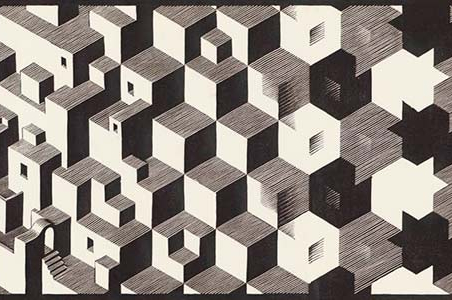
\includegraphics[scale=0.4]{escher.jpg}
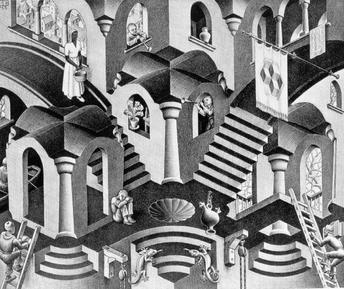
\includegraphics[scale=0.55]{escher2.jpg}
\caption{The Necker cube tiling as it appears briefly in ``Metamorphosis I," and impressed into a banner in ``Convex and Concave."[citation]}
\label{fig:Escher}
\end{center}
\end{figure}

Flat, periodic surfaces such as the Necker cube surface are of much interest to differential geometers for two reasons in particular. The first is that, locally, neighborhoods are isometric to the plane, making it remarkably easy to describe parallel transports between two points in tangent vector bundles over the surface by linear group actions. The second is that Riemann surfaces constructed out of infinitely many polyhedra can be \emph{flattened} and contained in the plane in such a way that the metric is preserved. The advantage in this case is that one obtains something akin to infinite billiard tables where a geodesic flows are represented by series of straight line segments in the plane. This paper will use such methods to prove dynamical results about Geodesic flows on the Necker cube surface.

\begin{rem}
Familiarity is assumed on the part of the reader with covering space theory, translation (Veech) surfaces, and their associated Veech groups. For general surveys on these topics: [cite], [cite].
\end{rem}

\subsection{Discussion of Results}
Our initial experiments strongly supported the theory that there would be a correlation between a choice of trajectory angle and dynamical properties of a geodesic on such a symmetric object. Rightfully so, a surface composed of infinitely many cubes an induced flat metric where every neighborhood is locally isometric to the Euclidean plane. Via the parallel transport of a unit tangent vector over the sharp edges of the surface, it becomes obvious to think of the geodesic as a sequence of line segments contained in the faces of each cube on the surface's embedded form in $\RR^3$. $\ref{fig:front}$.

\begin{wrapfigure}{l}{2.2in.}
\includesvg{vectorplane}
\end{wrapfigure}
\noindent Let $x_0$ be a point on the surface that is contained in an open neighborhood of a smooth section of the surface and consider a tangent unit vector $v\in\RR^3$ protruding from $x_0$. Assuming the faces are parallel to every $2$-dimensional subspace of $\RR^3$ spanned by standard basis vectors, exactly one component of $v$ would be 0. Projecting this vector to a parallel plane retains all necessary information about direction. Call this vector $v_0\in\RR^2$.
\\\\
We say that $v_0$ is the \emph{initial trajectory} of the geodesic and the angle it makes relative to our choice of basis is its \emph{initial trajectory angle}. We consider a rational direction to fall into one of two categories.
\begin{Def}
Let $v_0$ be a unit vector of the form $\frac{1}{k}(x,y)\in\RR^2$ with $x,y\in\mathbb{Z}$ and $k=\sqrt{x^2+y^2}\in\mathbb{R}$. We say $v_0$ is an \textbf{odd-odd} vector if its components are relatively prime and odd. We denote the \textbf{set of all odd-odd directions} by $\mathcal{O}$. We say that $v_0$ is an \textbf{even-odd} vector if its components are relatively prime and of opposite parity. We denote the \textbf{set of all even-odd directions} by $\mathcal{E}$.
\end{Def}
\noindent This paper will demonstrate how one reaches the following conclusion about the relationship between parity and periodicity of geodesic behavior on the Necker cube surface, denoted $\mathbf{S}$:

\begin{thm*}
(Directional Dichotomy of Periodic Geodesics on $\mathbf{S}$) Let $\Phi_t$ be a unit-speed geodesic flowing on the unit tangent bundle of $\mathbf{S}$ for $t\in\RR$ with initial point and vector $\Phi_0=(x_0,v)$. Then the following is true:
\begin{enumerate}[label=(\roman*)]
\item $\Phi$ is periodic with period $T\in\RR$ if and only if $v_0\in\cO$.
\item $\Phi$ is drift-periodic with period $T\in\RR$ if and only if $v_0\in\cE$.
\end{enumerate}
\end{thm*}

The proof for this theorem can be found in XXX and follows from Theorems YYYY and ZZZZZ.
\\
\compav{theorem about most directions being recurrent?}

\subsection{Acknowledgements}
-Pat Hooper\\
- Vincent Delecroix, Ferrán Valdez, pascal hubert\\
- \\

\newpage

\section{Periodic Tiling of Necker Cubes}
This section will detail how the Necker Cube surface is obtained as an infinite regular cover of a branched torus. Consider the Necker cube with the following identifications:
\begin{figure}[H]
\centering
\includesvg[width=2in.]{neckercube}
\end{figure}

We denote this surface $\bG$. $\bG$ is obtained by taking three copies of the unit square and identifying the edges in order to resemble the visible portion of a unit cube. $\bG$ is a genus one surface with three vertices homeomorphic to $\TT^2$. Check that every vertex has a cone angle of either $3\pi$ or $\frac{3\pi}{2}$. These are the conical singularities of the surface, $\Sigma$. We denote the surface without its singularities $\bG\backslash\Sigma = \bGs$. Thus, $\pi_1(\bGs)\cong\pi_1((thrice\text{-}branched~torus))\cong\pi_1(S^1\vee S^1\vee S^1\vee S^1)\cong\FF_4$, the free group of four generators.
\begin{Def}
The \textbf{Necker cube surface} $\mathbf{S}$ is obtained as the regular cover of $\bG$ by periodically tiling along the edges with solid triangles.\\
The \textbf{branched Necker cube surface} $\mathbf{S}^\circ$ is obtained similarly by tiling $\bGs$.
\end{Def}



\noindent Consider the following families of unit squares in $\RR^3$:\\
\vspace{0.2in}
\begin{tabular}{p{10cm}c}
\begin{align*}
\mathbf{A}_{m,n,p} = [m, m+1]\times[n,n+1]\times\{p\}, 
\\\mathbf{B}_{m,n,p} = \{m+1\}\times[n,n+1]\times[p-1,p],
\\\mathbf{C}_{m,n,p}= [m,m+1]\times\{n+1\}\times[p-1,p].
\end{align*}
&
\shiftleft{0.8in}{\raisebox{-1in}{
\includegraphics[scale=1]{label.png}}}
\end{tabular}

With the proper identifications on  $\mathbf{A}_{0,0,0}\cup\mathbf{B}_{0,0,0}\cup\mathbf{C}_{0,0,0}$, we have $\bG$'s embedded form in $\RR^3$ and a map $s:\bG\hookrightarrow\RR^3$. Similarly, removing the integer points from this set is an embedding of $\bGs$. Check that tiling along the edges as previously described determines a set of points in $\RR^3$ that coincides with points on $\mathbf{S}$ with $s^*$ as an extension of $s$ to the cover. That is, $s(\mathbf{S})=\bigcup\left\{\mathbf{A}_{m,n,p}\cup\mathbf{B}_{m,n,p}\cup\mathbf{C}_{m,n,p}~:~m+n+p=0\right\}$. Thus a point $x_0\in\mathbf{S}$ is in one-to-one correspondence with this set. To avoid ambiguity we say $U$ is a \emph{neighborhood} of $s(x_0)$ if it is contained in exactly one of $\mathbf{A}_{m,n,p}, \mathbf{B}_{m,n,p}, \mathbf{C}_{m,n,p}$. As $U$ must contain an open ball contained on a single square there cannot be a neighborhood where $s(x_0)\in\ZZ^3$ and $x_0$ is a conical point. It follows then that a neighborhood in $\mathbf{S}$ is a neighborhood in $\mathbf{S}^\circ$ as well. 

\begin{figure}[H]
\centering
\includesvg[width=1in]{cubesxyzcut}
\caption{A section of $\mathbf{S}$}
\end{figure}

\subsection{Flattening $\mathbf{S}$}
At the moment it is difficult to describe how the parallel transport of a vector tangent to the surface along an arbitrary path on the surface acts on the vector in $\RR^3$. To simplify this problem we take $\mathbf{S}$ to an isometric variant embedded in $\RR^2$ by piecewise linear transformations on the sets 
\begin{align*}
\mathbf{A}=\bigcup\big{\{}\mathbf{A}_{m,n,p}: m+n+p=0\big{\}},
\\\mathbf{B}=\bigcup\big{\{}\mathbf{B}_{m,n,p}: m+n+p=0\big{\}},
\\\mathbf{C}=\bigcup\big{\{}\mathbf{C}_{m,n,p}: m+n+p=0\big{\}}.
\end{align*}

\begin{Def}
Let $\Psi:s^*(\mathbf{S})\rightarrow\RR^3$ be given as
\begin{equation}
\Psi\left[\begin{array}{c}
	x\\y\\z
\end{array}\right] 
= 
\begin{cases}
	\left[ \hspace{2mm} \begin{matrix}
		1 & 0 & 0 \\
		0 & 1 & 0 \\
		0 & 0 & 1
	\end{matrix}\hspace{3mm}\right]

	\left[\begin{array}{c}
	x - \left\lfloor x \right\rfloor
	\\ y- \left\lfloor y \right\rfloor
	\\ -(z - \left\lfloor z \right\rfloor)
	\end{array} \right]
	+
	\left[\begin{array}{c}
		2 \left\lfloor x \right\rfloor - \frac{3}{2}
		\\ 2\left\lfloor y \right\rfloor - \frac{3}{2}
		\\ z - \left\lfloor z \right\rfloor
	\end{array} \right]
		& \text{if } (x,y,z)\in \mathbf{A}	\vspace{2mm}
	\\
		
		
	\left[ \begin{matrix}
	0 & 0 & 1 \\
	0 & 1 & 0 \\
	-1 & 0 & 0
	\end{matrix}\hspace{2mm}\right]
	\left[\begin{array}{c}
		x - \left\lfloor x \right\rfloor
		\\ y- \left\lfloor y \right\rfloor
		\\ -(z - \left\lfloor z \right\rfloor)
		\end{array} \right]
	+
		\left[\begin{array}{c}
			2 \left\lfloor x \right\rfloor - \frac{3}{2}
			\\ 2\left\lfloor y \right\rfloor - \frac{3}{2}
			\\ x - \left\lfloor x \right\rfloor
		\end{array} \right]
			& \text{if } (x,y,z)\in \mathbf{B}\backslash(\mathbf{A}\cup\mathbf{C})	\vspace{2mm}
	\\
	
		\left[ \begin{matrix}
		1 & 0 & 0 \\
		0 & 0 & 1 \\
		0 & -1 & 0
		\end{matrix}\hspace{2mm}\right]
		\left[\begin{array}{c}
			x - \left\lfloor x \right\rfloor
			\\ y- \left\lfloor y \right\rfloor
			\\ -(z - \left\lfloor z \right\rfloor)
			\end{array} \right]
		+
			\left[\begin{array}{c}
				2 \left\lfloor x \right\rfloor - \frac{3}{2}
				\\ 2\left\lfloor y \right\rfloor - \frac{3}{2}
				\\ y - \left\lfloor y \right\rfloor
			\end{array} \right]
				& \text{if } (x,y,z)\in \mathbf{C}\backslash(\mathbf{A}\cup\mathbf{B})	\vspace{2mm}
\end{cases}
\end{equation}
\end{Def}
\noindent This map behaves as such:
\begin{figure}[H]
\centering
\includesvg[width=1.1in]{cubesxyzcut} \hspace{0.1in}\raisebox{1.0in}{\text{$\rightarrow$}}\hspace{0.1in}
\raisebox{0.4in}{\includesvg[width=1.5in]{unfoldcut}}
\caption{An isometry of the surface $\mathbf{S}$.}
\label{fig:Psi}
\end{figure}

\begin{lem}
$\Psi\circ s^*$ is an isometry of the surface $\mathbf{S}$
\begin{proof}
$\Psi$ is well-defined on its domain $s^*(\mathbf{S})$, and $s^*$ is an embedding of the surface that is a bijection when restricting its co-domain to its image. Since $\Psi$ is a linear transformation composed of Euclidean matrices and translations it is also invertible and bijective. 
\end{proof}
\end{lem}

\subsection{Translation Surface Cover of $\bGs$}
Reconstruct $\bG$ and $\bGs$ to resemble a quotient of the flattened Necker cube surface by a series of cutting and gluing operations: \\
\begin{figure}[H]
\centering
\includesvg[width=3in]{LTorus}
\end{figure}
\noindent This L-shaped torus is then cut along the dotted lines and pieced together to look like a $2\times2$ torus with a unit square removed from the center:\\
\begin{figure}[H]
\centering
\includesvg[width=2in]{BranchTorus}
\caption{$\bGs$ with 4 independent, closed paths labeled identified}
\end{figure}
The paths labeled $a,b,c,d$ are independent. Let $\pi_1(\bGs)=\<a,b,c,d\>$. $\bGs$ has a $\ZZ^2$ tiling by traversing along paths $a,b$ and attaching infinitely many copies of the surface. It's apparent that this $\ZZ^2$ tiling is the flattened Necker cube surface. We use group homomorphisms on this free group to construct translation surfaces and $\ZZ^2$-covers to better understand geodesic behavior on the Necker cube surface.

\begin{Def}
Let $\varphi_1:\pi_1(\bGs)\rightarrow \ZZ^2$ be the group homomorphism defined on generators $a,b,c,d$: \\$c,d\mapsto(0,0)$\\ $a\mapsto(1,0)$\\$b\mapsto(0,1)$\\ $ab,ba\mapsto(1,1)$
\end{Def}

\begin{Def}
Let $\varphi_2:\pi_1(\bGs)\rightarrow SO(2,\ZZ)$ be the group homomorphism defined on the generators $a,b,c,d$:
\begin{align*}
a,b & \mapsto \begin{pmatrix}
1 && 0 \\ 0 && 1\end{pmatrix}=I_2\\
c & \mapsto\begin{pmatrix}0 && -1\\1 && 0\end{pmatrix}=R\\ d & \mapsto\begin{pmatrix}0 && 1\\-1 && 0\end{pmatrix}=R^3
\end{align*}
\end{Def}

Recall that a \emph{translation surface} is a compact, locally flat surface that admits a discrete number of conical singularities and has trivial linear holonomy on any arbitrary path. If the total cone angle of the singularity is some integer multiple of $2\pi$, $2\pi(d+1)$ for $d\geq 0$, we say that singularity has degree $d$. Two translation surfaces belong to the same stratum, or family, of surfaces characterized by the number and degree of conical singularities. Consider the effect that paths $c,d$ have on holonomy: 

\begin{figure}[H]
\centering
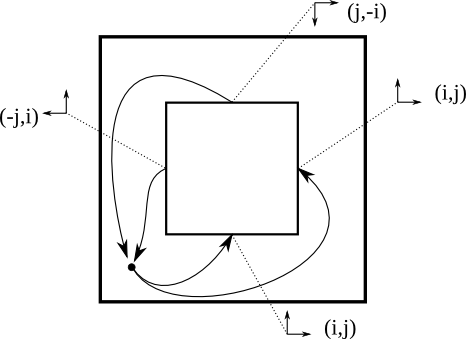
\includegraphics[width=2.5in]{monodromy.png}
\caption{Effect a nontrivial loop has on arbitrary basis vectors (i,j).}
\label{fig:loop}
\end{figure}

We construct a cover of $\bGs$ by taking four copies of it and cyclically pairing edges, and show that this cover has trivial holonomy. Denote the unit tangent bundle of $\bGs$ by $T^1\bGs$. Because $\bGs$ can be contained in the plane, we consider vectors tangent to $\bGs$ to be in $\RR^2$. Let $x_0\in\bGs$. The fiber over $x_0$ under the projection $T^1\bGs\twoheadrightarrow\bGs$ is the set $E_{x_0}$. Let $\triangledown$ be a flat metric connection on $T^1\bGs$ and $p=(x_0,v_0)\in E_{x_0}$ be a single element in the fiber over $x_0$ with $v_0\in\RR^2$. We denote the \emph{holonomy group} of the connection with base point $p$ by $Hol_p(\triangledown)=\{A\in SO(E_{x_0})~:~ p = A\cdot p\}$ where $p$ differs from $A\cdot p$ by some rotation of $v_0$. An element in $SO(E_{x_0})$ acts on $p$ by rotation of the vector $v_0$. Denote the \emph{holonomy bundle} based at $p$ by $H(p)=\{p'\in E_{x_0}~:~ p'= A\cdot p \}$, the set of elements in the orbit of $p$ where a closed loop $\gamma:[0,1]\rightarrow\bGs$ defines a horizontal lift to $\gamma^*:[0,1]\rightarrow T^1\bGs$ by parallel transport of $v_0$ along the path such that $p=\gamma^*(0)$, and $p'=\gamma^*(1)$. Since $\bGs$ is flat and trivial paths have trivial holonomy, $Hol_p(\triangledown)$ acts on $H(p)$ the monodromy group is discrete and well-defined on $\bGs$.

\begin{lem}
$\varphi_2:\pi_1(\bGs)\rightarrow \mathrm{SO}(2,\ZZ)$ is a monodromy representation of the surface.
\begin{proof}
It is clear from Figure 6 that this is the case as concatenating a closed loop with paths $c$ or $d$ would rotate a vector exactly by the cone angles of the singularities that they loops around: $\pm \frac{3\pi}{2}$.
\end{proof}
\end{lem}

\begin{Def}
Let $\bMs$ be the regular cover of $\bGs$ with fundamental group $\pi_1(\bMs)=\ker\varphi_2$.
\end{Def}
Showing that $\bMs$ is a degree four cover of $\bGs$ with trivial holonomy and deck group $\SO(2,\ZZ)$ follows immediately from its construction.
\begin{figure}[H]
\centering
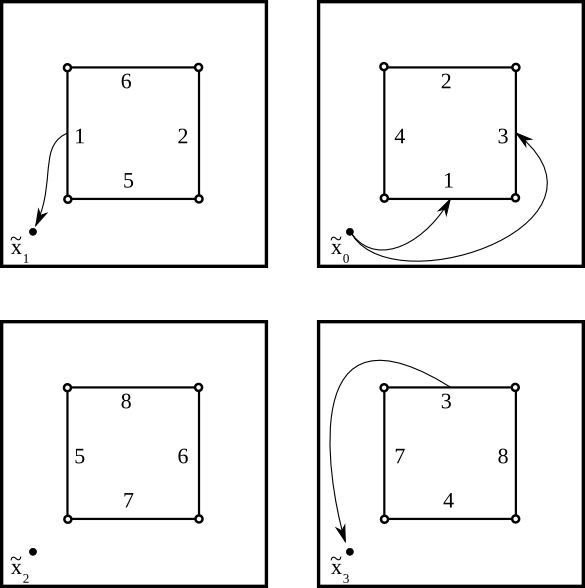
\includegraphics[width=3in]{monogroup.png}
\label{fig:arbitrarylift}
\caption{Lift of paths $c,d$ to $\bMs$ (\compav{RELABEL EDGES})}
\end{figure}

\begin{Def}
The surface $\bUs$ is the regular cover of $\bGs$ such that $\pi_1(\bUs)=\ker\varphi_1$. 
\end{Def}

The deck group of this cover is isomorphic to $\ZZ^2$. By reversing the cutting and gluing done previously to $\bGs$ and $\bG$, one can easily see that a cover defined as the kernel of this homomorphism is identical to the tiling of Necker cubes along two of its edges. For this reason, $\bU\cong\mathbf{S}$. 



\subsection{A Four-Fold Cover of $\bUs$}


\begin{figure}[H]
\centering
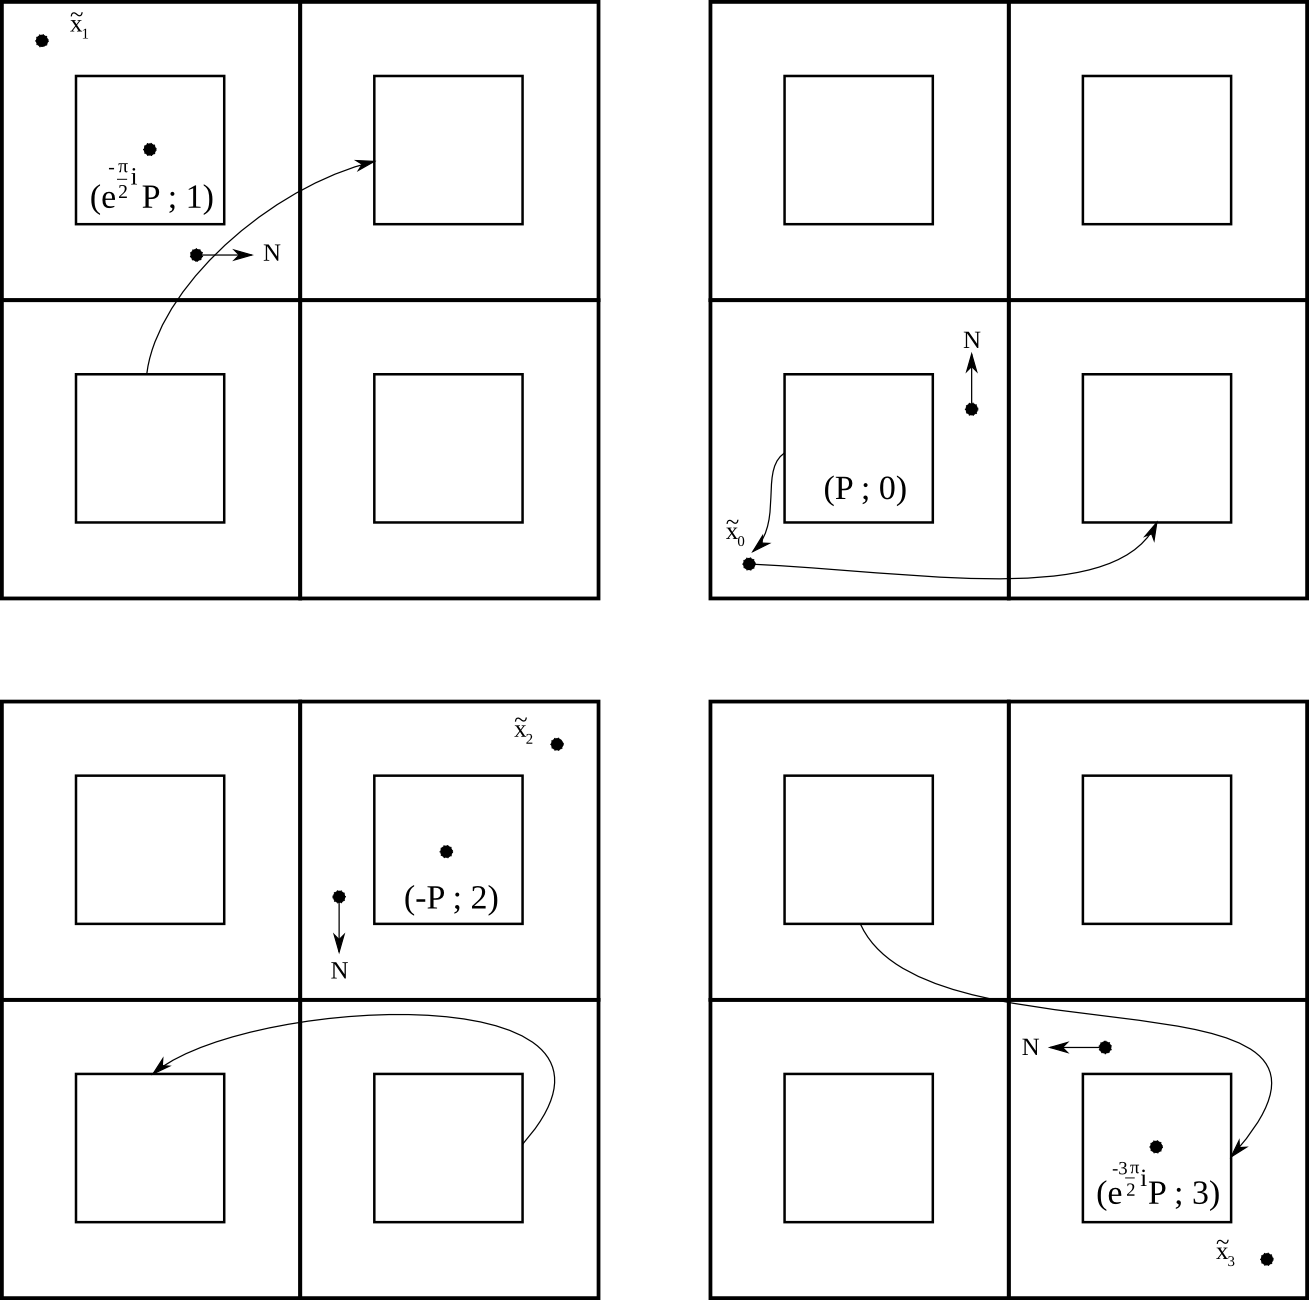
\includegraphics[width=3in]{coverdirection.png}
\end{figure}


\newpage
\begin{Def}
$\bUs$ is the cover of $\bGs$ such that $\pi_1(\bUs)=\ker\varphi$.
\end{Def}

Our cover of $\bGs$ has the fundamental group, $\pi_1(\bUs)=\<\<a^{-1}b^{-1}ab, c, d\>\>$, the conjugate subgroup of elements that map trivially under $\varphi_1$. The covering map $k_{\varphi_1}:\bUs\hookrightarrow\bGs$ takes every point on $\bUs$ to its modular equivalent under these translational symmetries. $\bUs$ is realized as an infinite $\ZZ^2$-tiling of $\bGs$ in $\CC$:
\begin{figure}[H]
\centering
\includesvg[width=2in]{uprime}
\caption{The infinite surface $\bUs$ embedded in $\CC$ with edges identified.}
\end{figure}

\begin{Def}
$\bU$ is the completion of $\bUs$ that includes the branched vertices. 
\end{Def}

\begin{rem}
The surface $\bG$ is homeomorphic to the torus, and its cover $\bU$ is its universal cover as the paths labeled $c,d$ are only non-trivial when $\bG$ is branched at its three conical points.
\end{rem}

\subsection{}

\subsection{Isometry From $\mathbf{S}$ to $\bU$}
The Necker cube surface can be \emph{flattened} onto the plane by piecewise isometric maps onto a subspace of $\RR^3$ with (open) unit squares removed at every even integer pair in the plane, what we claim to be $\bU$.

\noindent The red/blue dotted lines represent the edges that are split on the plane. The map from one surface to the other is composed of piecewise isometries, $\Psi:\mathbf{S}\rightarrow\RR^3$.



The flattened surface is contained entirely in $(x,y,0)\in\RR^3$, which is isometric to $\CC$. $\bU$ is recovered as a topological quotient on the domain

\begin{equation}
\label{eq:P}
\mathbf{P} = \mathbb{C}\text{ }\backslash\bigcup_{m,n \in {\mathbb Z}} \big{\{} u+vi:u\in(2m-\frac{1}{2},2m+\frac{1}{2}),\text{ } v\in(2n-\frac{1}{2},2n+\frac{1}{2})\big{\}}.
\end{equation}

\begin{Def} $\mathbf U$ is the surface obtained as the topological quotient $\mathbf{P}/\sim_{\mathbf{P}}$, where $\CC$ is identified with $\RR^2$ in the usual way and $\sim_{\mathbf{P}}$ is a minimal relation on $\mathbf{P}$ defined as follows:
\begin{gather*}
\text{Let } x_{0}=(u_{0},v_{0}),x_{1}=(u_{1},v_{1}) \in \mathbf{P}.  \text{ }\sim_{\mathbf{P}} \text { is given as the relation }\\ x_{0}\sim_{\mathbf{P}}x_{1}  \text{ iff } x_{0}=x_{1}
 \\\text{ or, for some }m,n\in\ZZ~x_{0},x_{1} \in {\partial} \left( \left[2m-\frac{1}{2},2m+\frac{1}{2}\right] \times \left[2n-\frac{1}{2},2n+\frac{1}{2}\right] \right)\\
  \left[\begin{array}{c}
u_{1} -2m
\\v_{1}-2n
\end{array}\right] = \left[\begin{matrix}
0 && 1\\
1 && 0
\end{matrix}\right]
\left[ \begin{array}{c}u_{0}-2m\\
v_{0}-2n
\end{array}\right]
.\end{gather*}\end{Def}

\begin{rem}
Our map $\Psi$ induces an isometry between $\mathbf{S}$ and $\bU$, and its restriction to the branched surfaces induces an isometry between $\mathbf{S}^\circ$ and $\bUs$. This follows from these piecewise Euclidean transformations that preserves our induced flat metric.
\end{rem}
From here on we use $\bUs$ and $\bU$ instead of $\mathbf{S}$ and $\mathbf{S}^\circ$.

\subsection{Four-Fold Cover}
We denote the \emph{unit tangent bundle} on the surface $\bUs$ by $T^1\bUs$, and construct a cover with trivial holonomy. Initial experiments have shown us that any geodesic viewed as discontinuous line segments on $\mathbf{P}$ moves in at most four directions.
\begin{figure}[H]
\centering
\includesvg[width=1.8in]{cubesxyzpaths}
\includesvg[width=2.8in]{unfoldcutpath}
\caption{Simple periodic (c) and drift-periodic (a,b) trajectories represented as line segments on $\mathbf{S}$ and $\mathbf{U}$.\compav{RELABEL THESE}}
\label{fig:holonomypath}
\end{figure}
Observe that the parallel transport of a vector around a closed loop on $\bUs$ will act on vectors tangent to the surface by a rotation of an integer multiple of $\frac{\pi}{2}$ radians (since the surface is flat and embedded in $\CC$, we work with vectors in $\RR^2$).



\begin{Def}
Define $\varphi_2:\pi_1(\bGs)\rightarrow SO(2,\ZZ)$ as the group homomorphism on generators $a,b,c,d$ such that:
\begin{align*}
a,b\mapsto \begin{pmatrix}1 && 0 \\ 0 && 1\end{pmatrix}=I_2,~~~
c\mapsto \begin{pmatrix}0 && -1 \\ 1 && 0\end{pmatrix}=R,~~~
d\mapsto \begin{pmatrix}0 && 1 \\ -1 && 0\end{pmatrix}=R^3
\end{align*}
\end{Def}
The homomorphism restricted to $\pi_1(\bUs)$ factors through $\pi_1(\bGs)$ and we show that:
\begin{lem}
The group $\varphi_2(\pi_1(\bUs,x_0))=Hol_p(\omega)$.
\begin{proof}
Since $c\mapsto R$ and $d\mapsto R^3$, the image of $\varphi_2$ is generated by $R,R^3$ and isomorphic to $SO(2,\ZZ)$. We see from figure $\ref{fig:holonomypath}$ that parallel transports of vectors by non-trivial paths produce clockwise/counter-clockwise rotations equal to that of of the cone angles of the singularities they loop around, all integer multiples of $\frac{\pi}{2}$ that coincide with paths generated by elements $c,d$. Further, if there is an element in $\pi_1(\bUs,x_0)$ conjugated by $[a,b]$, the effect this would have on holonomy would be trivial as the total cone angle sum around each cut out square is an integer multiple of $2\pi$, which agrees with $a$ and $b$'s trivial images under $\phi_2$.
\end{proof}
\end{lem}

Hence, we obtain a natural monodromy representation with the map $m:\pi_1(\bUs,x_0)\rightarrow SO(2,\ZZ)\cong Hol_p(\omega)$, where for $[\gamma]\in\pi_1(\bUs,x_0)$ we have that $\gamma^*(1)=(x_0,m([\gamma])v_0)$. It follows that since $\omega$ is a flat connection, trivial loops have trivial holonomy and $Hol_p(\omega)$ acts on $H(p)$.

\begin{figure}[H]
\centering
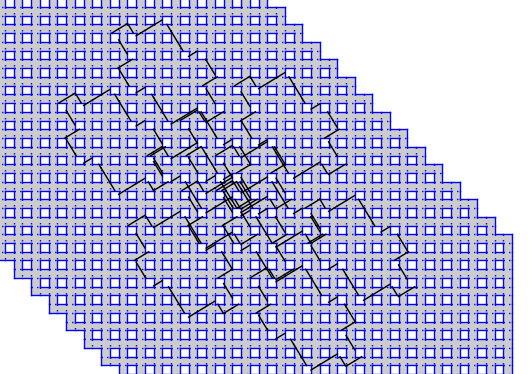
\includegraphics[width=4in.]{closed2.png}
\caption{Geodesic flow on $\mathbf{U}$ modeled using sage-flatsurf.}
\label{fig:complicated}
\end{figure}

\begin{Def}
Let $\btUos$ be the cover of $\bUs$ with fundamental group $\pi_1(\btUos)=\ker\varphi_2|_{\pi_1(\bUs)}\trianglelefteq \pi_1(\bUs)$.
\end{Def}

\begin{lem}
Let $\Phi_t:\bUs\times\RR\rightarrow \bUs$ be a unit-speed geodesic flow on $\bUs$, with a parallel transport map induced by $\omega$. Then the following is true:
\begin{enumerate}[label=(\roman*)]
\item $\Phi$ is periodic if and only if its lift to $\btUos$ is.
\item $\Phi$ is drift-periodic if and only if its lift to $\btUos$ is. 
\end{enumerate}
\begin{proof}
Let $x_0=\Phi(0)$ be an initial point in $\bUs$, and let $v_0=\frac{d}{dt}\Phi|_{t=0}\in\RR^2$ be its initial direction. Then $\Phi^*:T^1\bUs\times\RR\rightarrow T^1\bUs$ is a well-defined lift to the unit tangent bundle with initial point $p=(x_0,v_0)$.
\\\emph{(i)}. Suppose $\Phi$ is periodic with period $T\in\RR$. Then $\Phi$ is reparameterized as $\alpha:[0,1]\rightarrow \bUs$, where $[\alpha]\in\pi_1(\bUs,x_0)$. It follows then that if $\alpha$ does not lift to a closed path, then $\alpha$ must have non-trivial holonomy since $[\alpha]\notin\ker\varphi_2$. That is when lifted to the unit tangent bundle with base point $p$, $\alpha^*(1)\neq p$ since $m([\alpha])\neq I_2$. But this implies that $\Phi^*(T)\neq p$, which is impossible. Hence $[\alpha]\in\ker\varphi_2=\pi_1(\btUos,\tilde{x}_0)$, where $\tilde{x}_0$ belongs to the fiber over $x_0$ under the covering map $\btUos\hookrightarrow\bUs$. The converse holds trivially.
\\\emph{(ii)}. Suppose $\Phi$ is drift-periodic with period $T\in\RR$ and non-trivial $f:\bUs\rightarrow\bUs \in Trans(\bUs)\cong\pi_1(\bGs)/\pi_1(\bUs)\cong \ZZ^2$ such that $\Phi(T)=f(x_0)$. Re-parameterize this as $\alpha:[0,1]\rightarrow\bUs$ with $[\alpha]\in\pi_1(\bGs)$.  When lifted to $T^1\bUs$, $\Phi^*(0)=p$ and $\Phi^*(T)=(f(x_0),v_0)$. Let $\alpha:[0,1]\rightarrow \bUs$ be its reparameterization up to time $T$. Thus $[\alpha]\notin \pi_1(\bUs,x_0),\pi_1(\btUos,\tilde{x}_0)$. Further, $f$ has a unique, lift to $\tilde{f}\in Trans(\btUos)$ because the space is connected. (a bit stuck here). \\
Conversely, ...
\end{proof}
\end{lem}


A visual representation of $\btUos$ is as a four-fold cover of $\bUs$ with trivial holonomy on all closed paths. Arbitrary paths do \emph{not} have trivial holonomy:



\begin{figure}[H]
\centering
\includesvg[width=1.5in.]{quotient}
\caption{A $2\times2$ cut out section centered at each missing square. Edges and vertices identified.}
\label{fig:quotient}
\end{figure}

\subsection{Translation Surface}

A better picture of $\btUos$ is obtained by making cyclic edge identifications on $\mathbf{P'}=\mathbf{P}\times\ZZ/4\ZZ$. This comes from $\btUos$ inheriting the topological properties of $\bUs\times \pi_1(\bUs)/\pi_1(\btUos)\cong \bUs\times SO(2,\ZZ)$.


\begin{figure}[H]
\centering
\includesvg[width=4in]{utilda}
\label{fig:utilda0}
\caption{Branched cover of $\mathbf{U}$ of degree four.}
\end{figure}

\begin{Def}
$\btU_0$ is the surface obtained as the quotient $\mathbf{P}'/\sim_{\mathbf{P}'}$. Denote paths $\zeta$ and $\eta$  on $\mathbf{P}$, parameterized by integers $m,n\in\ZZ$ and $t\in[-\frac{1}{4},\frac{1}{4}]$, and defined:\\ $\zeta(t)=(2m+t)+i(2n-\frac{1}{2})$,\\
$\eta(t)=(2m+t)+i(2n+\frac{1}{2})$.\\ Let $\aleph=2m+i2n\in\CC$. The minimal relation $\sim_{\mathbf{P}'}$ is given as:
\begin{equation}
\begin{split}
(\zeta(t);j)\sim_{\mathbf{P'}}(e^{i\frac{\pi}{2}}~\overline{\zeta(t)-\aleph};j+1)\\
(\eta(t);j)\sim_{\mathbf{P'}}(e^{i\frac{\pi}{2}}~\overline{\eta(t)-\aleph};j+1)
\label{eq:rel2}
\end{split}
\end{equation}
\end{Def}
This relation is similar to $\sim_\mathbf{P}$ in that it translates line segments of squares surrounding even integer pairs to the origin and relates points on one edge of a square to points on an adjacent edge. Where it differs is that these adjacent edges now belong to a different ``copy" of $\mathbf{P}$. It is in this cyclic manner that edges are glued that allows for trivial linear holonomy on arbitrary paths by rotating each copy of $\mathbf{P}$ accordingly. For example, here is a path on a section of the surface in the neighborhood of $P=2m+i2n\in\CC$ $(m,n\in\ZZ)$ after rotation:



\noindent and its subsequent projection onto $\bUs:$

\begin{figure}[H]
\centering
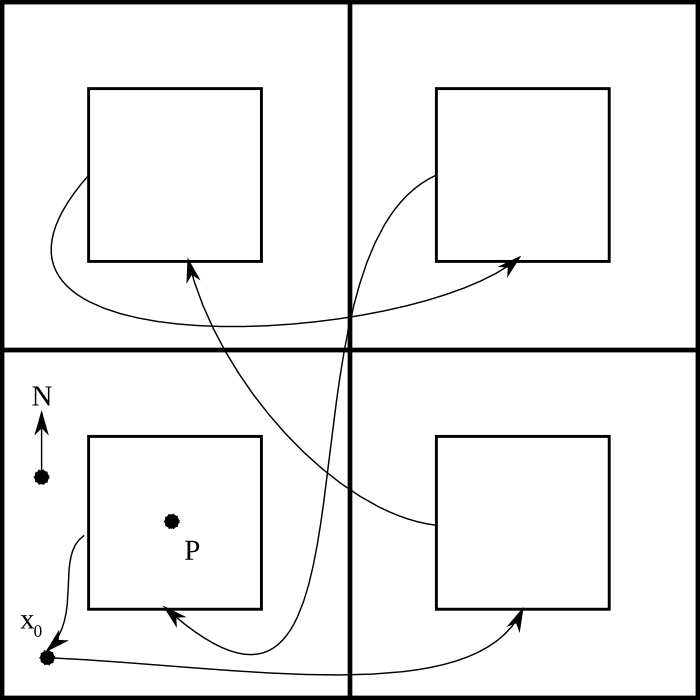
\includegraphics[width=2in]{overlay.png}
\end{figure}

\begin{Def}
Let $r:\mathbf{P}'\rightarrow\mathbf{P}'$ be the isometric map of $\btU_0$'s domain given  $r(z;\bar{j})=(e^{(-j)i\frac{\pi}{2}}z;\bar{j})$.
\end{Def}

Observe that when $r$ acts on the relations $\eqref{eq:rel2}$ we get the following:

\begin{equation}
\begin{split}
(e^{(-j)i\frac{\pi}{2}}\zeta(t);j)\sim_{r(\mathbf{P'})}(e^{(-j)i\frac{\pi}{2}}~{\zeta(t)-\aleph};j+1)\\
(e^{(-j)i\frac{\pi}{2}}\eta(t);j)\sim_{r(\mathbf{P'})}(e^{(-j)i\frac{\pi}{2}}~{\eta(t)-\aleph};j+1)
\end{split}
\end{equation}

$\btU$ is then recovered as $r\cdot(\btU_0)=\mathbf{P'}/\sim_{r(\mathbf{P}')}$, where all identifications are translations made on copies of $\mathbf{P}$.
\subsection{Veech Staircase Model}
Let $f:\btU\rightarrow\mathbf{M}$ be a projection onto the quotient surface that takes every point to its modular equivalent by its $\ZZ^2$ symmetries, and what we obtain is the following compact translation surface belonging to the stratum $\cH(2,2,2,2):$

\begin{figure}[H]
\centering
\includesvg[width=2.6in]{mtilda}
\caption{Compact translation surface, $\mathbf{M}$, covered by the infinite surface with edges and cone singularities (1,2,3,4) identified. The Roman numerals are meant to identify each quotient with a plane in the cover, $\mathbf{\tilde{\mathbf{U}}}$.}
\label{fig:mtilda}
\end{figure}

We rearrange $\bM$ as such:

\begin{figure}[H]
\centering
\includesvg[width=3.4in]{mtildastaircase}
\caption{The staircase Veech surface with directional planes and vertices identified. All edges are paired by translation. Two adjacent squares have opposite edges identified. The top edge of the bottom-left square is glued to the bottom edge of the top-right square (both labeled I). Likewise, the bottom edge of the bottom-left square is identified with the top edge of the top-right square.}
\label{fig:staircase}
\end{figure}

\noindent We recall some basic definitions and theorems about $\ZZ^2-$covers of translation surfaces as they apply to $\bM$. 

\begin{Def}
Algebraic intersection number is a non-degenerate bilinear form:
\begin{align*}
i:H_1(\bM,\QQ)\times H_1(\bM,\QQ)\rightarrow\QQ,
\end{align*}
for $[\gamma],[\beta]\in H_1(\mathbf{M},\QQ)$, $i([\beta],[\gamma])$ returns the signed intersection number of two homology classes. We say a crossing at the instance of an intersection is positive if $\gamma$ makes a positive angle relative to $\beta$. 
\end{Def}
The set of all affine diffeomorphisms of $\bM$ form the group $\text{Aff}^+(\bM)$. The $\emph{Veech group}$ of $\bM$ is the image in the co-domain of the homomorphism $D:\text{Aff}^+(\bM)\rightarrow SL(2,\RR)$ that takes every affine map to its derivative, which we denote $V(\bM)$. $\bM$ is a square-tiled translation surface whose Veech group is a finite index subgroup of $SL(2,\ZZ)$. We use automorphisms of the fundamental group in $\text{Aut}(\pi_1(\bM))$ induced by affine maps to prove our main results. But first, we define a group homomorphism from $\pi_1(\bM)$ to $\pi_1(\bM)/\pi_1(\btU)$ by algebraic intersection numbers pver a sum of linearly independent homology classes. Consider the following cylinder core curves on $\bM$ labeled $\gamma_i$ for $0\leq i\leq 11$:
\begin{figure}[H]
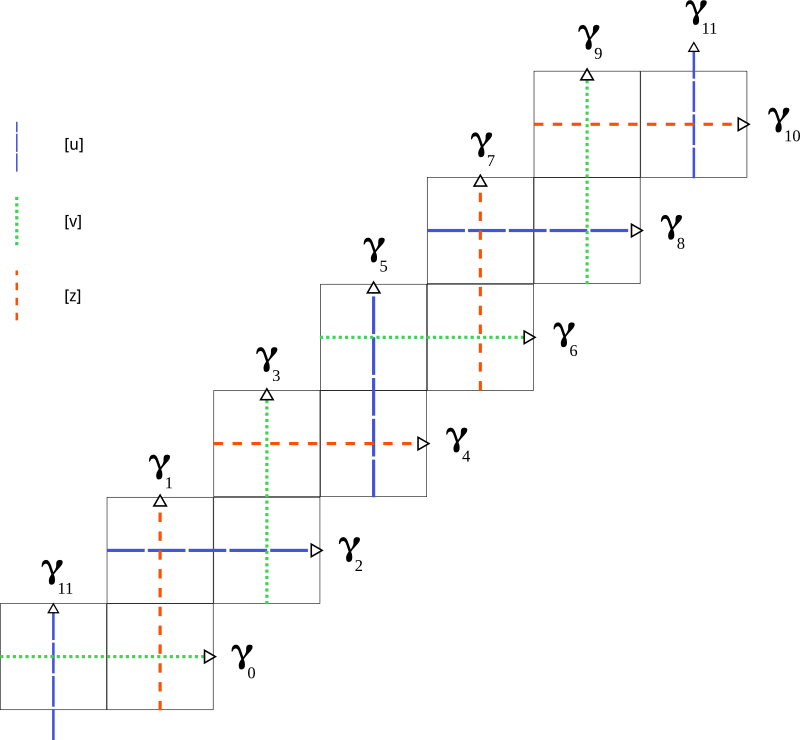
\includegraphics[width=3in]{homologyclass.png}
\centering
\caption{$\bM$'s cylinder core curves with u,v, and z homology class labels.}
\label{fig:homology}
\end{figure}

Every curve intersects two others and if we take $i(\Sigma_{i=0}^{11}[\gamma_i])$
\compav{show that $\gamma_0,\dots,\gamma_{11}$ form a basis for $H(\bM,\QQ)$}\\
\compav{show that u,v linearly independent}


\begin{Def}
The homology classes $u,v,z$ are given as the following sums of core curves:
\begin{align*}
u &= -[\gamma_2] +[\gamma_5] + [\gamma_8] - [\gamma_{11}],\\
v &= +[\gamma_0] -[\gamma_3] -[\gamma_6] +[\gamma_9],\\
z &= +[\gamma_1] +[\gamma_4]-[\gamma_7]-[\gamma_{10}].
\end{align*}
\end{Def}

\begin{Def}
Define the group homomorphism $\Omega_{u,v}:\pi_1(\bM)\rightarrow \QQ^2$, where $\beta\mapsto(i(u,[\beta]),i(v,[\beta]))$.
\end{Def}

\begin{lem} $\Omega_{u,v}(\pi_1(\bM))=\ZZ^2$.
\end{lem}
\begin{lem}
\compav{show somehow that u,v determine the cover}
\end{lem}

\subsection{Induced Automorphisms of $H_1(\bM,\QQ)$}
We look at some important automorphisms induced by Affine maps on $\bM$. Observe that $\bM$ has a uniform cylinder decomposition in both horizontal and vertical directions as in figure $15$. We define the \emph{modulus}, $\mu$, of a cylinder to be the ratio of the cylinder's width to its circumference, $\frac{w}{c}$. The $\emph{Dehn-twist}$ of a cylinder is an affine diffeomorphism that skews the cylinder and sends every vertex to itself.

\begin{figure}[H]
\centering
\includesvg[width=3in]{cylinderskew}
\label{fig:skew}
\caption{Dehn-twist of a cylinder in $\bM$'s cylinder decomposition.}
\end{figure}

Such a map would have derivative $\left[~\begin{matrix}1 && \pm\mu^{-1}\\0 && 1\end{matrix}~\right]$. On $\bM$ every cylinder in both vertical and horizontal decompositions has a modulus of $\frac{1}{2}$. These give way to global diffeomorphisms as $\emph{multi-twists}$ of $\bM$.

\begin{Def}
We call the global affine diffeomorphisms in $\text{Aff}^+(\bM)$ obtained as \textbf{multi-twists of the surface in horizontal and vertical directions} $\mathbf{A}$ and $\mathbf{B}$, respectively.
\\We define the \textbf{derivatives of} $\mathbf{A},\mathbf{B}$ as the matrices 
$D(\mathbf{A})=\mathbf{A}'=\left[ \hspace{1mm} \begin{matrix}
				1 &   2\\
				0 & 1
			\end{matrix}\hspace{1mm}\right] \text{ , and }
			D(\mathbf{B})=\mathbf{B}'=\left[ \hspace{1mm} \begin{matrix}
							1 & 0\\
							 2 & 1
						\end{matrix}\hspace{1mm}\right]$, where $D:\text{Aff}^+(\bM)\rightarrow V(\bM)$.
\end{Def}
These are parabolic elements of $V(\bM)$ that are directly related to the dynamical dichotomy of rational trajectories on the Necker cube surface. To show this algebraically, we look at how skewing the surface affects our homology spanning core curves:

\begin{figure}[H]
\centering
\includesvg[width=2in]{skew}
\end{figure}

When skewing the surface under $\mathbf{A}$ in the horizontal direction, the horizontal curves are preserved, but the vertical curves (odd $\gamma_i$ index) obtain two additional positive intersections with adjacent index (mod 12) horizontal curves. Similarly, the vertical $\mathbf{B}$ skews preserve the vertical curves, but the horizontal curves (even $\gamma_i$ index) obtain two additional \emph{negative} intersections with adjacent index (mod 12) vertical curves. The formulaic expressions of the $\mathbf{A}, \mathbf{B}$ induced automorphisms of $H_1(\bM,\QQ)$ as powers of $k\in\ZZ$ are then:

\begin{align*}
\mathbf{A}^k_*([\gamma_i])=&[\gamma_i] + \frac{k}{2}(1-(-1)^i)([\gamma_{i-1}]+[\gamma_{i+1}])\\
\mathbf{B}^k_*([\gamma_i])=&[\gamma_i] + \frac{k}{2}(1+(-1)^i)([\gamma_{i-1}]+[\gamma_{i+1}])\\
\end{align*}

With all of these in mind we generate the following subgroups:

\begin{Def}
We say $\XX$ is the subgroup of $\text{Aff}^+(\bM)$ generated by $\mathbf{A}$, $\mathbf{B}$.
\end{Def}

\begin{Def}
The images of $\XX$ under their derivative maps to $V(\bM)$ is the subgroup of $V(\bM)$ generated by matrices $\mathbf{A}',$ $\mathbf{B}'$. We denote this group by $\XX'$.
\end{Def}

\begin{Def}
The induced automorphisms of $\XX$ contained in $Aut(H_1(\bM,\QQ))$ is the subgroup generated by $\mathbf{A}_*$, $\mathbf{B}_*$.
\end{Def}
\section{Proof of Main Theorem}

\subsection{Translation Surfaces and $\ZZ^2$-Covers}


\begin{Def}
Algebraic intersection number is a non-degenerate bilinear form:
\begin{align*}
i:H_1(S,\mathbf{R})\times H_1(S,\mathbf{R})\rightarrow\mathbf{R},
\end{align*}
where $\mathbf{R}$ is a ring and for $[\gamma],[\beta]\in H_1(S,\mathbf{R})$, $i([\beta],[\gamma])$ returns the intersection number of two homology classes.
\end{Def}
Algebraic intersections are signed and follow some convention such as the right-hand rule.

\begin{Def}
Let $u,v\in H_1(S,\QQ)$ be linearly independent homology classes of curves on $S$. Then the group homomorphism from $\pi_1(S)$ to $\QQ^2$ is given as:
\begin{align*}
\Omega_{u,v}:\pi_1(S)\rightarrow \mathbf{R}^2 \text{; } \beta\mapsto(i(u,[\beta]),i(v,[\beta])).
\end{align*}
\end{Def}



The set of all orientation-preserving affine diffeomorphisms of $S$ forms the group Aff$^+(S)$. The corresponding \emph{Veech group}, $V(S)$ of $S$ is the image of the group morphism $D:\text{Aff}^+(S)\rightarrow SL(2,\mathbb{R})$ that takes an affine map to its derivative. A surface is said to be \emph{Veech} if its Veech group is commensurable to $SL(2,\mathbb{R})$. It is well known that origami, or square-tiled, surfaces have Veech groups commensurable to $SL(2,\ZZ)$. [cite] When $\mathbf{R}=\ZZ$, $\Omega_{u,v}$ takes an element of $\pi_1(S)$ to $\Delta$. Thus, $\gamma\in\pi_1(S)$ lifts to $\tilde{\gamma}\in\pi_1(\tilde{S})$ if and only if $\gamma\in\ker\Omega_{u,v}$.

\begin{Def}
Let $\alpha:[0,1]\rightarrow S$ be a closed, non-singular geodesic path on $S$. The holonomy map $\mathbf{hol}:H_1(S, \mathbf{R})\rightarrow\CC$ returns the holonomy vector of a closed path as a difference of the starting and endpoints of a flow by\\
\begin{align*}
\mathbf{hol}([\alpha])=\int_{\alpha}dz.
\end{align*}
\end{Def}
Since $\alpha$ is non-singular, it can be mapped to $S^\circ$ which admits a flat holomorphic one-form $dz$. Let $\theta=Arg(\mathbf{hol}([\alpha]))$. We say that $\phi_t^\theta:\RR\times S^\circ \rightarrow S^\circ$ is the unit-speed geodesic flow on $S^\circ$ in direction $\theta$ given by the  $[\alpha]$ such that $\phi^\theta_0=\alpha(0)$. In local coordinates this corresponds to $z+te^{i\theta}\in \CC$.

\begin{lem}
$\phi_t^\theta$ has a period of $T=|\mathbf{hol}([\alpha])|$
\begin{proof}
This just follows from the fact that $\phi_t^\theta$ flows at unit-speed in the direction of $\frac{\mathbf{hol}([\alpha])}{|\mathbf{hol}([\alpha])|}$. 
\end{proof}
\end{lem}
And so the length of a vector determines the period of a flow on $S$. More importantly, we have the following:

\begin{lem}
Denote the lifted flow of $\phi_t^\theta$ on $\tilde{S}$ by $\tilde{\phi}_t^\theta$. Then $\tilde{\phi}_t^\theta$ is periodic on $\tilde{S}$ and $\tilde{S}^\circ$ if and only if $[\alpha]\in\ker\Omega_{u,v}$. Further, $\tilde{\phi}_t^\theta$ has period $T=|\mathbf{hol}([\alpha])|$.
\begin{proof}
Suppose that $[\alpha]\notin\ker\Omega_{u,v}$. Since $\alpha([0,1])=\phi^\theta_{[0,\hol([\alpha])]}$, their homology classes are equivalent. Hence $\tilde{\phi}_t^\theta$ could not close on $\tilde{S}$ or $\tilde{S}^\circ$, or else $\Omega_{u,v}(k[\alpha])=k(i(u,[\alpha]),i(v,[\alpha]))=(0,0)$ for some non-zero $k\in\ZZ$. Conversely, suppose $[\alpha]\in\ker\Omega_{u,v}$. Then 
\end{proof}
\end{lem}

\begin{cor}
If $[\alpha]\notin\ker\Omega_{u,v}$, then $\tilde{\phi}_t^\theta$ is drift-periodic with period $T=\hol([\alpha])$.
\begin{proof}
This follows immediately from the previous lemma since $\tilde{S},\tilde{S}^\circ$ have translational $\ZZ^2$ symmetries and a well-defined $\ZZ^2$ action on an element in the fiber of a basepoint in $S$ under $f$. The period is $T$ since a geodesic closes on $S$ with period $T$.
\end{proof}
\end{cor}

\begin{lem}
Let $h\in\text{Aff}^+(S)$. If $h(\beta)=\alpha$ for closed geodesics $\alpha,\beta$ on $S$ and $\beta$ lifts to a closed path on $\tilde{S}$, then so does $\alpha$. (not sure about this)
\begin{proof}
If the premise is true, then $[\beta]\in\ker\Omega_{u,v}$. Denote the group automorphism induced by $h$ as $h_*$. Then $\Omega_{u,v}([\alpha])=\Omega_{u,v}([h(\beta)])=\Omega_{u,v}(h_*\cdot[\beta])=(i([\beta],h_*^{-1}\cdot u),i([\beta],h_*^{-1}\cdot v))=(0,0)$ as automorphisms .
\end{proof}
\end{lem}

\begin{lem}
Let $\beta=h(\alpha)$ as before. If $D(h)=h'\in V(S)$ and $S$ is Veech, then $\tilde{\phi}^\theta_t$ has period $T=h'\cdot\hol([\beta])$. (also not sure)
\begin{proof}

\end{proof}
\end{lem}



\subsection{Symmetries of $\bM$}



\section{Four-fold Cover of $\mathbf{U}$}

\begin{figure}[H]
\centering
\includesvg[width=2.05in.]{fourfold}\hspace{0.5in}\includesvg[width=2.05in.]{fourfoldrotate}
\caption{Four-fold cover isometry and the preimage of a point in $\mathbf U \backslash Sing(\mathbf U)$.}
\end{figure}

\begin{figure}[H]
\centering
\includesvg[width=3.15in]{utilda}
\label{fig:utilda0}
\caption{Branched cover associating every direction with one plane.}
\end{figure}

\begin{figure}[H]
\centering
\includesvg[width=3.15in]{utildaprime}
\caption{Infinite-type translation surface obtained by rotating each copy of the fundamental domain accordingly.}
\label{fig:utilda}
\end{figure}

The quotient under the group action of translational symmetries is isomorphic to $\mathbb{Z}^2$ since the orbit of any point in the fundamental domain is a lattice in the space. 

\begin{thm}
The translational symmetries of $\tilde{\mathbf{U}}$'s fundamental domain induce symmetries on the surface isomorphic to $\mathbb{Z}^2$.
\begin{proof}
Let $(z;j)\in\mathbb{C}\times\mathbb{Z}/4\mathbb{Z}$ and define the group action $T_0^{m,n}:\mathbb{C}\times\mathbb{Z}/4\mathbb{Z}\rightarrow\mathbb{C}\times\mathbb{Z}/4\mathbb{Z}$ as $T^{m,n}(z;j)=(z+2e^{-j\frac{i\pi}{2}}(m+in);j)$. This translation acts faithfully on the preimages of $\mathbf{U}\backslash Sing(\mathbf{U})$, and respects edge identifications of $\mathbf{\tilde{\mathbf{U}}}$, thereby making it an isometry of the surface. Consider a group homomorphism, $T_0^{m,n}\mapsto m+in$ onto the plane of Gaussian integers, $\mathbb{Z}[i]$. The exponential function is never zero, so the identity of the translation group is $T_0^{0,0}$. This is an isomorphism since it is clearly surjective and any non-trivial element of $T^{m,n}$ could not possibly map to the identity element of $\mathbb{Z}[i]$, regardless of the value of j. Since $\mathbb{Z}^2$ is isomorphic to $\mathbb{Z}[i]$, it is isomorphic to  $T_0^{m,n}$ as well.
\end{proof}
\label{thm:z2}
\end{thm}


\begin{Def}
The automorphism $T^{m,n}:\tilde{\mathbf{U}}\rightarrow\tilde{\mathbf{U}}$ is an  \textbf{induced translation} of $\tilde{\mathbf{U}}$ as a result of the previous theorem.
\end{Def}




This surface is obtained as a ramified cover of the unit square torus. It is a translation surface and is therefore equipped with a \textbf{holomorphic one-form}, a collection of charts from neighborhoods of $\mathbf{M}$ to $\mathbb{C}$ such that any neighborhood away from Sing$(\mathbf{M})$ has a \emph{flat} induced Euclidean metric. A theorem of Gutkin and Judge tells us that its Veech group is commensurable to SL$(2,\mathbb{Z})$ and is therefore a Veech surface. We look at some of its affine maps, and generate a subgroup $\mathbb{X}\subset$ Aff$^+(\mathbf{M})$  by the following transformations:


\begin{enumerate}[label=(\roman*)]
\item Multi-twists of the surface as global diffeomorphisms given by Dehn-twists of its cylinder decomposition in horizontal and vertical directions with derivatives:
\begin{equation*}
\left\{ \left[ \hspace{1mm} \begin{matrix}
				1 &  \pm 2\\
				0 & 1
			\end{matrix}\hspace{1mm}\right] \text{ , }
			\left[ \hspace{1mm} \begin{matrix}
							1 & 0\\
							 \pm 2 & 1
						\end{matrix}\hspace{1mm}\right] \right\}.
\end{equation*}
we call $\mathbf{A}^{\pm 1}$, $\mathbf{B}^{\pm 1}$, respectively.\\
A Dehn-twist on each cylinder in the cylinder decomposition of $\mathbf{M}$ in horizontal and vertical directions gives way to these global affine diffeomorphisms:


\item Rotation group generated by a $+\frac{\pi}{2}$ rotation of the surface fixed about the center of the second square on the bottom of the staircase, an order four isometry on $\mathbf{M}$ denoted $\mathbf{R}$.

\item  Order 2 translation of the surface that moves the bottom left-most square to the square right next to it, denoted $\mathbf{H}$.
\item Order 2 translation of the surface that takes the bottom right-most square to the one right above it, denoted $\mathbf{V}$.
\end{enumerate}

\begin{Def}
The group $\mathbb{X}$ is the isometry group generated by affine maps $\mathbf{A}$,$\mathbf{B}$,$\mathbf{R}$, $\mathbf{H}$, and $\mathbf{V}$. The image of the derivative map on elements in $\mathbb{X}$ is denoted $\mathbb{X}'$ and generated by matrices
\begin{align*}
\left[\begin{matrix}
1 & 2 \\ 0 & 1
\end{matrix}\right],
\left[\begin{matrix}
1 & 0 \\ 2 & 1
\end{matrix}\right],
\left[\begin{matrix}
0 & -1 \\ 1 & 0
\end{matrix}\right],
\end{align*}
denoted $\mathbf{A}'$, $\mathbf{B}'$, and $\mathbf{R}'$ in that order.
\end{Def}

It is not immediately apparent if these affine maps generate Aff$^{+}(\mathbf{M})$, or if their derivatives generate $V(\mathbf{M})$, its Veech group. We use these to induce homomorphisms on $H_1(X, \mathbb Q)$. A spanning set of $H_1(\mathbf{M}, \mathbb Q)$ is obtained as the set of homology classes of the core curves of X's cylinder decompositions in both vertical and horizontal directions:

\begin{figure}[H]
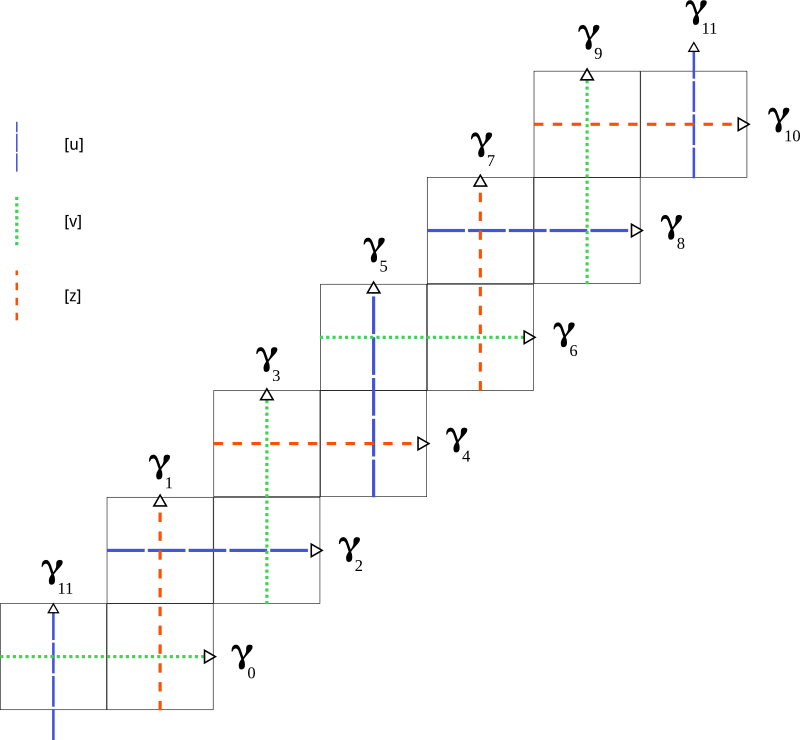
\includegraphics[width=3in]{homologyclass.png}
\centering
\caption{Cylinder core curves with u,v, and z homology classes that determines the $\mathbf{Z}^{2}$-cover.}
\label{fig:homology}
\end{figure}

\begin{Def}
The set of abelianized cylinder core curves is denoted as $\Gamma=\{\gamma_i: i = 0,\dots,11\}\subset H_1(\mathbf{M},\mathbb{Q})$.
\end{Def}

\begin{rem}
We use 12 elements to span homology, although a basis requires only 10. It's not impossible to determine the relations between these core curve classes, but it is not necessary. A $12\times12$ matrix of these core curve cylinder decompositions to their intersection numbers with adjacent curves is rank 10, as to be expected.
\end{rem}

The induced homomorphisms of $H_1(\mathbf{M}, \mathbb Q)$ have come from affine maps that have various effects on these core-curves. We use a 12-gon to represent the set of curves, and show how these elements act on them. The multi-twists add curves to adjacent curves, and the translation maps permute them. The reader is encouraged to check these for themselves.

e.g. for $\mathbf{H,V}\in$Aff$^+(\mathbf{M})$,

\begin{minipage}{0.5\textwidth}
\vspace{0.3in}
\begin{itemize}
\item[\textbf{\emph{$\mathbf{H}$ \& $\mathbf{V}$}}] The effect that these two translations have on the 12-gon is a reflection about these lines. Observed by keeping track of the squares and core curves after $\mathbf{H}$ and $\mathbf{V}$ have acted on $\mathbf{X}$.
\end{itemize}
\end{minipage}
\begin{minipage}{0.7\textwidth}
\begin{figure}[H]
\hspace{0.2in}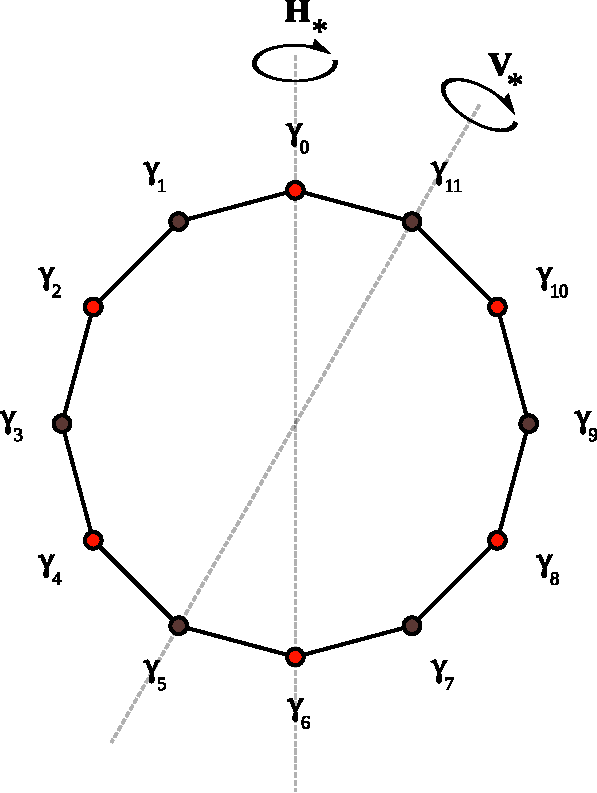
\includegraphics[width=1.7in]{12gonHV.pdf}
\end{figure}
\end{minipage}

\begin{Def}
The induced homomorphisms of $H_1(\mathbf{M},\mathbb{Q})$ are obtained from the affine subgroup $\mathbb{X}$ and denoted $\mathbb{X}_*$. The associated homomorphisms on the spanning set $\Gamma$ are given as:
\begin{align*}
\mathbf{A}^k_*\circ[\gamma_i]=&[\gamma_i] + \frac{k}{2}(1-(-1)^i)([\gamma_{i-1}]+[\gamma_{i+1}])\\
\mathbf{B}^k_*\circ[\gamma_i]=&[\gamma_i] + \frac{k}{2}(1+(-1)^i)([\gamma_{i-1}]+[\gamma_{i+1}])\\
\mathbf{R}_*\circ[\gamma_i]=&(-1)^i[\gamma_{1-i\text{ mod }12}]\\
\mathbf{H}_*\circ[\gamma_i]=&[\gamma_{12-i\text{ mod }12}]\\
\mathbf{V}_*\circ[\gamma_i]=&[\gamma_{10-i\text{ mod }12}]
\end{align*}
\end{Def}

\begin{Def}
The homology classes $u,v,z$ are given as the following sums of core curves:
\begin{align*}
[u] &= -[\gamma_2] +[\gamma_5] + [\gamma_8] - [\gamma_{11}],\\
[v] &= +[\gamma_0] -[\gamma_3] -[\gamma_6] +[\gamma_9],\\
[z] &= +[\gamma_1] +[\gamma_4]-[\gamma_7]-[\gamma_{10}].
\end{align*}
\end{Def}

\begin{thm}
The fundamental group of the $\mathbb{Z}^2$-cover is obtained by lifting the kernel of the closed paths of $\mathbf{M}$ of the homomorphism:

\begin{align*}
\Omega_{u,v}:\pi_1(\mathbf{M},x_0)\rightarrow \mathbb{Z}^2 \text{; } \beta\mapsto(i(u,[\beta]),i(v,[\beta])),\text{ where}
\end{align*}

\begin{align*}
i:H_1(\mathbf{M},\mathbb Q)\times H_1(\mathbf{M},\mathbb Q)\rightarrow \mathbb Z.
\end{align*}is the intersection number of two homology classes.
\begin{proof}
We know from Theorem $\ref{thm:z2}$ that the translational symmetries of $\tilde{\mathbf{U}}$ induced by $T^{m,n}$ is isometric to $\mathbb{Z}^2$. Since $\mathbf{M}$ is a genus 5 base surface, we know that $\pi_1(\mathbf{M},x_0)\simeq \mathbb{Z}^{10}$, and the associated cover satisfies $\mathbf{M}=\tilde{\mathbf{U}}/(\pi_1(\mathbf{M},x_0)/N)$, such that $N$ is a normal subgroup of $\pi_1(\mathbf{M},x_0)$. This means that $N\simeq \mathbb{Z}^8$. The eight core curve classes are the abelianized forms of  $\gamma_0,\gamma_2,\gamma_3,\gamma_5,\gamma_6,\gamma_8,\gamma_9,$ and $\gamma_{11}$ that span N. The classes and their signs are obtained from Figure $\ref{fig:mtilda}$ as the outer regions identified by the translations of $T^{m,n}$. Thus any closed path on $\mathbf{M}$ is lifted to a closed path on the cover under the quotient map only when a path has a trivial intersection number with the classes.
\end{proof}

\end{thm}
Two paths are homologous if they return the same intersection number with the classes of closed core cylinder curves of $\mathbf{U}$ that span its homology. The classes u and v are obtained from the group group action of $T^{m,n}$ on the cover.

\begin{Def}
$\mathbf{hol}:\mathbf{M}\backslash\text{Sing}(\mathbf{M})\rightarrow\mathbb{C}$ is the holonomy vector pulled back from a non-singular path $\gamma$ in $\mathbf{M}$ onto the complex plane given by $\mathbf{hol}(\gamma)=\int_{\gamma}dz$.
\end{Def}

We denote the \textbf{closed path} $\alpha$, such that $\mathbf{hol}(\alpha)=6+6i$, and show it is homologous to the closed geodesic with the same holonomy vector. The slope one direction also decomposes $\mathbf{M}$ into two cylinders by a series of saddle connections of length $\sqrt{2}$ between singularities:

\begin{figure}[H]
\centering
\includesvg[width=4.4in.]{slopeonecylinder}
\caption{The two right-most cylinders $C_1$ (labeled) and $C_2$(unlabeled).}
\end{figure}

The circumferences of these two cylinders are $6\sqrt{2}$. Geodesic flows on this surface are well defined, and rational directions 

\begin{Def}
Let $\omega^{\theta}_t:[0,1]\times\mathbb{R}/2\pi\mathbb{Z}\rightarrow\mathbf{M}$ be the \textbf{maximal geodesic flow} on the surface in direction $\theta$ such that $\omega^{\theta}_0=\omega^{\theta}_1=x_0\in\mathbf{M}\backslash\text{Sing}(\mathbf{M})$.\\
$\omega^{\frac{\pi}{4}}_t$ is the geodesic flow in the \textbf{slope one direction}, and $\chi$ is its image in $\mathbf{M}$ and element of $\pi_1(\mathbf{M},x_0)$.
\end{Def}

\begin{lem}
$\alpha$ is homologous to $\chi$ in  $\mathbf{M}\backslash\text{Sing}(\mathbf{M})$.
\begin{proof}
Let $\chi$ be a geodesic contained in either $C_1$ or $C_2$. Since a geodesic does not admit singularities, it is the image of a closed path on $X\backslash\text{Sing}(X)$ with initial point $x_0$ on the strips of $C_1$ and $C_2$ with boundaries removed, denoted $C_1',$ $C_2'$. Express $[\alpha]$ as $\Sigma^{11}_{j=0}$ $\frac{1}{2}\gamma_j$ (a closed path climbing up the staircase). We show that the intersection numbers of $[\alpha]$ and $[\chi]$ are the same for every core cylinder curve $\gamma$, i.e. $i([\gamma_k], \Sigma^{11}_{j=0} \text{ } \frac{1}{2}[\gamma_j])=i([\gamma_k],[\chi])\text{ } \forall k=0,\dots,11$.\\
\textbf{Case one:} k is even. If k is even, then every curve $\gamma_k$ is oriented to the right. Since $\chi$ intersects every curve once, $i([\gamma_k],[\chi])=1$. No even indexed curves intersect eachother, so we need only consider when $j$ is odd. Now if $j$ is odd, it is incident (positively crossing) with only two horizontal curves, namely $\gamma_{j+1},\gamma_{j-1}$. Therefore $i([\gamma_k],[\alpha])=i([\gamma_{j-1}],\frac{1}{2}[\gamma_{j}])+i([\gamma_{j+1}],\frac{1}{2}[\gamma_{j}])=\frac{1}{2}(i([\gamma_{j-1}],[\gamma_{j}])+i([\gamma_{j+1}],[\gamma_{j}]))=\frac{1}{2}(1+1)=1.$\\
\textbf{Case two:} k is odd. If k is odd, then $[\chi]$ will have an intersection number of $-1$ with $[\gamma_k]$ since odd-indexed core curves are oriented upwards. Now since k is odd, we only consider when $j$ is even. Similarly, this means that $\gamma_j$ negatively intersects the two vertical core curves with adjacent indices. Hence, $i([\gamma_k],[\alpha])=i([\gamma_{j-1}],\frac{1}{2}[\gamma_{j}])+i([\gamma_{j+1}],\frac{1}{2}[\gamma_{j}])=\frac{1}{2}(i([\gamma_{j-1}],[\gamma_{j}])+i([\gamma_{j+1}],[\gamma_{j}]))=\frac{1}{2}(-1-1)=-1.$\\
We know intersection number to be bilinear and non-degenerate on homology. So if $\alpha$ and $\chi$'s abelianizations admit the same intersection numbers for every curve in the spanning set of $H_1(\mathbf{M}, \mathbb{Q})$, then $[\alpha]=[\chi]$.
\end{proof}
\end{lem}

\begin{thm}
$\chi\in\pi_1(\mathbf{M},x_0)$ lifts to $\tilde{\chi}\in\pi_1(\tilde{\mathbf{U}},\tilde{x}_0)$
\begin{proof}
From Lemma 2, $[\chi]=[\alpha]$, so $\Omega_{u,v}(\chi)=\Omega_{u,v}(\alpha)$. Since
$i([u],[\alpha])=-i([\gamma_2],[\alpha] +i([\gamma_5],[\alpha]) + i([\gamma_8],[\alpha]) - i([\gamma_{11}],[\alpha])=-1+(-1)+1-(-1)=0$ and $i([v],[\alpha])=1-(-1)-1+(-1)=0$, it follows that $\alpha,\chi\in\text{Ker }\Omega_{u,v}$, and $\chi$ lifts to a closed geodesic on $\tilde{\mathbf{U}}$.
\end{proof}
\end{thm}

\begin{cor}
content...
\end{cor}

From here, we use $\alpha$ to show that the \emph{only} trajectories that close on the Necker cube surface are those that are in vector direction $(a,b)$ such that $\gcd(a,b)=1$ and $a,b$ are both odd. We call these \textbf{odd-odd} directions. We can make this claim because the group generated by the matrices 

\begin{equation*}
\left[ \hspace{1mm} \begin{matrix}
				1 &  \pm 2\\
				0 & 1
			\end{matrix}\hspace{1mm}\right] \text{ and }
			\left[ \hspace{1mm} \begin{matrix}
							1 & 0\\
							 \pm 2 & 1
						\end{matrix}\hspace{1mm}\right]
\end{equation*}
is the \emph{Sanov subgroup} of $SL(2,\mathbb{Z})$ and only sends elements in the odd-odd set to itself. There are dualizations made between how these matrices skew a geodesic direction,  and how their original affine transformations induce an effect homology. In a sense the kernel is obtained by the orbit of $\chi$ under $\mathbb{X}$ and its holonomy vector under $\mathbb{X}'$.

\begin{lem}
The actions of $\mathbb{X}'$ on $\mathcal{O}$ and $\mathcal{E}$ are closed in their respective sets.
\begin{proof}
Since $\mathbb{X}'$ is generated by the elements $\mathbf{A}'$, $\mathbf{B}'$, and $\mathbf{R}'$, any matrix $G'\in\mathbb{X}'$ is of the form $G' = (\mathbf{A}')^{1_1}\circ(\mathbf{B}')^{1_2}\circ(\mathbf{R}')^{1_3}\circ(\mathbf{A}')^{2_1}\circ\dots(\mathbf{A}')^{n_1}\circ(\mathbf{B}')^{n_2}\circ(\mathbf{R}')^{n_3}$, where $i_k\in\mathbb{Z}$ for $i=1,\dots,n$ and $k=1,2,3.$ Let $x=\left(\begin{matrix}p \\ q  \end{matrix}\right),y\in\mathcal{O}$, and consider the equation $G'x=y$. Observe that $\left(\begin{matrix}1 && 2 \\ 0 && 1\end{matrix}\right)^l x=\left(\begin{matrix}p+2jq \\ q  \end{matrix}\right),$ and $ \left(\begin{matrix}1 && 0 \\ 2 && 1\end{matrix}\right)^m x=\left(\begin{matrix}p \\ q+2mp  \end{matrix}\right)$ for any $l,m\in\mathbb{Z}$. Also note that for any $j\in\mathbb{Z}$, $(\mathbf{R}')^{m}x=\left(\begin{matrix}p \\ q  \end{matrix}\right),\left(\begin{matrix}-q\\ p  \end{matrix}\right),\left(\begin{matrix}-p \\ -q  \end{matrix}\right),\left(\begin{matrix}q \\ -p  \end{matrix}\right)$ when $j \mod{4}\equiv0,1,2,3$, respectively. In any case, the product of any power of a generator of $\mathbb{X}'$ and any $x\in\mathcal{O}$ is an element of $\mathcal{O}$ . By letting $l=i_1,m=i_2,$ and $j=i_3$, we first consider the base case when $i=n$. Let $G'=G'_1\circ\dots\circ G'_n$, such that $G'_i=(\mathbf{A}')^{i_1}\circ(\mathbf{B}')^{i_2}\circ(\mathbf{R}')^{i_3}$. Since $n_1,n_2,n_3$ are arbitrary integers, $G'_n x \in\mathcal{O}$. Suppose for some $b< n-1$, $G'_{n-b}\circ\dots\circ G'_n x =y'\in\mathcal{O}$. Therefore $y'=(G'_1\circ\dots\circ G'_{b})^{-1}y$, which implies that $(G'_1\circ\dots\circ G'_{b})^{-1}$ preserves the set $\mathcal{O}$. Otherwise, if $y\in\mathcal{E}$, there exists at least one $G'_i$ for $1< i< b$ and $\tau\in\mathcal{E}$ such that $G'^{-1}_i \tau = (\mathbf{R}')^{-i_3}\circ(\mathbf{B}')^{-i_2}\circ(\mathbf{A}')^{-i_1} \tau \in \mathcal{O}$, a contradiction. Since elements in $\mathbb{X}'$ are invertible, $G'_1\circ\dots\circ G'_{b}$ must also map $\mathcal{O}$ to itself. Left multiply both sides of the equation to show that $G'_1\circ\dots\circ G'_n x = G' x = y$. By the principle of strong induction, this holds for all $0<b\leq n$. Since $G'$ is invertible and an arbitrarily chosen element of $\mathbb{X}'$, it follows that $x\in\mathcal{O}$ if and only if $y\in\mathcal{O}$ and $\mathcal{O}$ is closed under $\mathbb{X}'$.\\
The proof for when $x\in\mathcal{E}$ is made in the same way.
\end{proof}
\end{lem}


Now a trajectory in the horizontal direction has a directional vector of (1,0). The orbit of this vector by the Veech group is the set of all \textbf{even-odd} vectors. We also know that in this direction a geodesic is drift-periodic (See figure 1). The Veech group of $\mathbf{M}$ preserves these properties. Suppose you had some closed geodesic on $\mathbf{M}\backslash Sing(\mathbf{M})$ called $\beta$ such that $\beta=h(\alpha)$, where $h\in$  Aff$^+(\mathbf{M})$, and $h_*$ is its induced homomorphism. Then we want to show that

\begin{align*}
(i([\beta],[u]), i([\beta],[v]))=(i([\alpha],h^{-1}_*[u]), i([\alpha],h^{-1}_*[v])) = (0,0).
\end{align*}

But first, we look at some of the properties of the group $\mathbb{X}_*$.

\begin{thm}
Let $\mathbb{X}_*$ be the group generated by $\mathbf{A}_*, \mathbf{B}_*, \mathbf{R}_*, \mathbf{H}_*,$ and $\mathbf{V}_*$. Let $G=\left< \mathbf{A}_*, \mathbf{B}_* \right>$, $T=\left< \mathbf{H}_*, \mathbf{V}_* \right>$, and $R=\left< \mathbf{R}_*\right>$. Then the following is true:
\begin{enumerate}[label=(\roman*)]
\item $G$ is a free subgroup of $\mathbb{X}_*$ of rank two.
\item $T$ is a finite cyclic subgroup of $\mathbb{X}_*$ and a centralizer of G.
\item $R$ is a finite cyclic subgroup of $\mathbb{X}_*$, and a normalizer of $G$.
\end{enumerate}
\begin{proof} Let $h_*^{j}=\mathbf{A}_*^{k_j}\circ \mathbf{B}_*^{g_j}\in G$ for $k_j, g_j \in\mathbb{Z}$, $j=1,\dots,n$.\\ \emph{(i)}. When $\mathbf{A}_*$ and $\mathbf{B}_*$ act on $\gamma_i$, it is only ever trivial if i is even for $\mathbf{A}_*$ or i is odd on $\mathbf{B}_*$. Since i cannot be both odd and even at the same time, there is no relation between the two generators and therefore $G$ is free.\\
\emph{(ii)} It is up to the reader to show that $T$ has the relations $\mathbf{H}_*^2=\mathbf{V}_*^2=(\mathbf{H}_*\mathbf{V}_*)^3=id_*$, and is isomorphic to the rotational group of the hexagon generated by reflections about adjacent vertices of a 12-gon. Observe that $\mathbf{H}_*\circ \mathbf{A}_*^{k_j}\circ[\gamma_i]=\mathbf{H}_*\circ[\gamma_i] + \frac{k_j}{2}(1-(-1)^i)(\mathbf{H}_*\circ[\gamma_{i-1}]+\mathbf{H}_*\circ[\gamma_{i+1}])=[\gamma_{-i}] + \frac{k_j}{2}(1-(-1)^i)([\gamma_{1-i}]+[\gamma_{-i-1}])=\mathbf{A}^{k_j}\circ[\gamma_-i]=\mathbf{A}^{k_j}\circ\mathbf{H}_*\circ[\gamma_i],$ and $\mathbf{V}_*\circ \mathbf{A}_*^{k_j}\circ[\gamma_i]=\mathbf{V}_*\circ[\gamma_i] + \frac{k_j}{2}(1-(-1)^i)(\mathbf{V}_*\circ[\gamma_{i-1}]+\mathbf{V}_*\circ[\gamma_{i+1}])=[\gamma_{10-i}] + \frac{k_j}{2}(1-(-1)^i)([\gamma_{11-i}]+[\gamma_{9-i}])=\mathbf{A}^{k_j}\circ[\gamma_10-i]=\mathbf{A}^{k_j}\circ\mathbf{V}_*\circ[\gamma_i].$ In the same way one can show this to be true for $\mathbf{B}_*^{g_j}$, and we can see that $T$ is a centralizer of $G$. \\
\emph{(iii)} $R$ is obviously cyclic and finite since an isomorphism is obtained as $\mathbf{R}_*\mapsto\mathbf{R}'\in SO(2,\mathbb{Z})$. \\Note that $\mathbf{R}_*\circ\mathbf{A}_*^{k_j}\circ[\gamma_i]=\mathbf{R}_*\circ[\gamma_i] + \frac{k_j}{2}(1-(-1)^i)(\mathbf{R}_*\circ[\gamma_{i-1}]+\mathbf{R}_*\circ[\gamma_{i+1}])\\
=(-1)^i[\gamma_{1-i}] + \frac{k_j}{2}(1-(-1)^i)((-1)^{i-1}[\gamma_{2-i}]+(-1)^{i+1}[\gamma_{-i}])\\
=(-1)^{1-i}([\gamma_{1-i}] - \frac{k_j}{2}(1+(-1)^{1-i})([\gamma_{2-i}]+[\gamma_{-i}]))\\
=(-1)^{1-i}\mathbf{B}_*^{-k_j}\circ[\gamma_{1-i}]=\mathbf{B}_*^{-k_j}\circ(-1)^{1-i}[\gamma_{1-i}]=\mathbf{B}_*^{-k_j}\circ\mathbf{R}_*\circ[\gamma_{i}].$\\
Likewise, $\mathbf{R}_*\circ\mathbf{B}_*^{g_j}\circ[\gamma_{i}]=\mathbf{A}_*^{-g_j}\circ\mathbf{R}_*\circ[\gamma_{i}]$.
\end{proof}
\end{thm}

\begin{rem}
It can be easily shown that $\mathbb{X}'$ has similar properties.
\end{rem}


\begin{lem}
$Let$ $h_*\in \left<\mathbf{A}_*,\mathbf{B}_*\right>. $ Then $h_*\circ[\alpha]\in H_1(\mathbf{M},\mathbb{Q})$ can be expressed as $h_*\circ[\alpha]=\frac{1}{2}(c_1\Sigma^{5}_{j=0}[\gamma_{2j}]+c_2\Sigma^{5}_{j=0}[\gamma_{2j+1}])$ for $c_1,c_2\in\mathbb{Z}$.
\begin{proof}
Let $\Sigma^{5}_{j=0}[\gamma_{2j}]=\Sigma\Gamma_{even}$, $\Sigma^{5}_{j=0}[\gamma_{2j+1}]= \Sigma\Gamma_{odd}$, and  $\Sigma^{11}_{j=0}[\gamma_{j}]= \Sigma\Gamma$. Let $h_*=h_*^n\circ\dots\circ h_ *^1$, and $h_*^{i}=\mathbf{A}_*^{k_i}\circ \mathbf{B}_*^{g_i}$ for $k_i, g_i \in\mathbb{Z}$, $i=1,\dots,n$. Compose these two homomorphisms and obtain $\mathbf{A}_*^{k_i}\circ \mathbf{B}_*^{g_i}(\Sigma\Gamma)=(4g_ik_i+2k_i)\Sigma\Gamma_{even}+2g_i\Sigma\Gamma_{odd}+\Sigma\Gamma$. Let $c_i^1=(4g_ik_i+2k_i), c_i^2=2g_i$, and solve for $h_*^{i+1}\circ h_*^i\circ\Sigma\Gamma$:
\begin{align*}
h_*^{i+1}\circ h_*^{i}\circ(\Sigma\Gamma)=h_*^{i+1}\circ(c_i^1\Sigma\Gamma_{even}+c_i^2\Sigma\Gamma_{odd}+\Sigma\Gamma)\\ =c_i^{1}h_*^{i+1}\circ(\Sigma\Gamma_{even})+c_i^2h_*^{i+1}\circ(\Sigma\Gamma_{odd})+h_*^{i+1}\circ(\Sigma\Gamma)\\ =2g_{i+1}\Sigma\Gamma_{odd}+(4g_{i+1}k_{i+1}+2k_{i+1})\Sigma\Gamma_{even}+\Sigma\Gamma\\+c_i^{1}(4g_{i+1}k_{i+1}\Sigma\Gamma_{even}+2g_{i+1}\Sigma\Gamma_{odd}+\Sigma\Gamma_{even})\\+c_{i}^2(2k_{i+1}\Sigma\Gamma_{even}+\Sigma\Gamma_{odd})\\
=\Sigma\Gamma+(c_i^1+(c_{i}^1+1)(4g_{i+1}k_{i+1})+(c_i^2+1)2k_{i+1})\Sigma\Gamma_{even}\\+(c_i^2+(c_i^1+1)2g_{i+1})\Sigma\Gamma_{odd}\\
\text{Let }c_{i+1}^1:=(c_i^1+(c_{i}^1+1)(4g_{i+1}k_{i+1})+(c_i^2+1)2k_{i+1}),\\
c_{i+1}^2:=(c_i^2+(c_i^1+1)2g_{i+1}).
\end{align*}
From these recursive definitions and a finite sequence of integers, $\{k\}_i,\{g\}_i$, observe then that\\ $h_*\circ[\alpha]=h_*\circ[\frac{1}{2}\Sigma\Gamma]=\frac{1}{2}h_*\circ[\Sigma\Gamma]=\frac{1}{2}[c_n^1\Sigma\Gamma_{even}+c_n^2\Sigma\Gamma_{odd}+\Sigma\Gamma]\\
=\frac{1}{2}[(c_n^1+1)\Sigma\Gamma_{even}+(c_n^2+1)\Sigma\Gamma_{odd}]$. Further simplify by letting $c_1=c_n^1+1,c_2=c_n^2+1$.
\end{proof}
\end{lem}

\begin{lem}
Let $h_*\circ[\alpha]\in H_1(\mathbf{M},\mathbb{Q})$. Then for $a\in\left<\mathbf{H}_*, \mathbf{V}_*\right>$ and $b\in\left<\mathbf{R}_*\right>$, the following is true:
\begin{align*}
& a\circ h_*\circ[\alpha]=h_*\circ[\alpha]\\
& b\circ h_*\circ[\alpha]=\frac{1}{2}[c'_1\Sigma\Gamma_{even}+c'_2\Sigma\Gamma_{odd}]\\
& h_*\circ b\circ[\alpha]=\frac{1}{2}[c''_1\Sigma\Gamma_{even}+c''_2\Sigma\Gamma_{odd}]
\end{align*}
\begin{proof}
By Theorem 4, a is a centralizer of the group so $a\circ h_*\circ[\alpha]=h_*\circ a \circ[\alpha]=h_*\circ \frac{1}{2}a \circ[\Sigma\Gamma].$ Since a is a cyclic permutation of the set $\Gamma$, it acts trivially on $\Sigma\Gamma$. Therefore, $a\circ h_*\circ[\alpha]=h_*\circ \frac{1}{2}[\Sigma\Gamma]=h_* \circ[\alpha]$.\\
By theorem 4, $a\circ\mathbf{A}_*^{k_i}\circ\mathbf{B}_*^{g_i}=\mathbf{B}_*^{-k_i}\circ\mathbf{A}_*^{-g_i}\circ a$. Extend this property to $h_*$, and denote the normalized element as $h_{**}$, such that $b\circ h_{*}=h_{**}\circ b$.  Note that $b(\Sigma\Gamma)=b(\Sigma\Gamma_{even}+\Sigma\Gamma_{odd})=\Sigma\Gamma_{odd}-\Sigma\Gamma_{even}$. $b\circ h_*\circ[\Sigma\Gamma]=c_1b\circ\Sigma\Gamma_{even}+c_2b\circ\Sigma\Gamma_{odd}=c_1\Sigma\Gamma_{odd}-c_2\Sigma\Gamma_{even}.$ So, $c_1'=-c_2$ and $c_2'=c_1$.\\
Since $h_*$ is arbitrary, let $h_{**}=g_{*}$ be generated by an integer sequence that defines the word and consider $h_*\circ b\circ[\Sigma\Gamma]=b\circ g_{*}\circ[\Sigma\Gamma]=c^*_1b\circ\Sigma\Gamma_{even}+c^*_2b\circ\Sigma\Gamma_{odd}=c^*_1\Sigma\Gamma_{odd}-c_2^*\Sigma\Gamma_{even}.$ So, $c_1''=-c_2^*$ and $c_2''=c_1^*$.
\end{proof}
\end{lem}

\noindent Now that every element in the orbit of $[\alpha]$ can be expressed as a linear combination of integers, it is simple to show they lift to a closed trajectory in the cover.

\begin{Def}
Let $\mathbf{dir}:UT(\mathbf{M}\backslash\text{Sing}(\mathbf{M}))\rightarrow\mathcal{O}\cup\mathcal{E}$ be the injective map from $\mathbb{R}/2\pi\mathbb{Z}$ to $\mathbb{Z}^2$ given as $\mathbf{dir}(\theta)=(k_1\cos(\theta),k_2\sin(\theta)), k_1,k_2\in\mathbb{R}$ such that $\gcd(k_1\cos(\theta),k_2\sin(\theta))=1$.
\end{Def}

\begin{thm}(Sketch)\\
Any geodesic, $\beta$, in $\mathbf{M}$ lifts to a closed geodesic $\tilde{\beta}$ on $\tilde{\mathbf{U}}$ if and only if $\mathbf{dir}(Arg(\mathbf{hol}(\beta)))\in\mathcal{O}$.
\begin{proof}
Call the quotient cover $p:\tilde{\mathbf{U}}\rightarrow\mathbf{M}$, and fix a point $\tilde{x_0}\in p^{-1}(x_0)$. Let $\beta=h(\chi)$, where $h\in\mathbb{X}$. We also obtain $[\beta]=h_*\circ[\alpha]$ from Lemma 2. Since $h$ sends geodesics to geodesics, h induces the following: $\mathbf{hol}(h(\chi))=h'(\mathbf{hol}(\chi))=h'(6+6i)$ for $h'=\left[\begin{matrix} a & b \\ c & d\end{matrix}\right]\in\mathbb{X}'$. So, Arg$(h'(\mathbf{hol}(\chi)))=$Arg$(6[(a+b)+i(c+d)])=$Arg$(6h'(1+i))$. Lemma 3 states that for any $h'\in\mathbb{X}'$, $h'(\mathcal{O})=\mathcal{O}$. Therefore there is no such geodesic of \textbf{even-odd} slope in the orbit of $\chi$. Otherwise $h',h\notin\mathbb{X}',\mathbb{X}$. Consequently, $\mathbf{dir}(Arg(\mathbf{hol}(\beta)))\in\mathcal{O}$.\\
From Lemma 5 we see that $[h(\chi)]=h_*\circ[\chi]=h_*\circ[\alpha]=\frac{1}{2}(c_1\Sigma^{5}_{j=0}[\gamma_{2j}]+c_2\Sigma^{5}_{j=0}[\gamma_{2j+1}])$ for $c_1,c_2\in\mathbb{Z}$. Denote the sums as $\Sigma\Gamma_{even}$ and $\Sigma\Gamma_{odd}.$\\
Therefore, $2i([u],h_*\circ[\alpha])=c_1i([u],\Sigma\Gamma_{even})+c_2i([u],\Sigma\Gamma_{odd})\\
=c_1(-i([\gamma_2],0) +i([\gamma_5],[\gamma_6]+[\gamma_4]) + i([\gamma_8],0) - i([\gamma_{11}],[\gamma_{10}]+[\gamma_{0}]))\\
+c_2(-i([\gamma_2],[\gamma_1]+[\gamma_3]) +i([\gamma_5],0) + i([\gamma_8],[\gamma_7]+[\gamma_9]) - i([\gamma_{11}],0))\\
=c_1(-(0)+(-1-1)+(0)-(-1-1))+c_2(-(1+1)+(0)+(1+1)-(0))=0.$\\\vspace{0.1in}\\
Similarly, $2i([v],h_*\circ[\alpha])=c_1i([v],\Sigma\Gamma_{even})+c_2i([v],\Sigma\Gamma_{odd})\\
=c_1(i([\gamma_0],0)-i([\gamma_3],[\gamma_2]+[\gamma_4])-i([\gamma_6],0)+i([\gamma_9],[\gamma_8]+[\gamma_{10}])\\
+c_2(i([\gamma_0],[\gamma_{11}]+[\gamma_1])-i([\gamma_3],0)-i([\gamma_6],[\gamma_5]+[\gamma_7])+i([\gamma_9],0)\\
=c_1((0)-(-2)-(0)+(-2))+c_2((2)-(0)-(2)+(0))=0.$\\
Therefore, $\Omega_{u,v}(h(\chi))=(0,0)$, and $h(\chi)=\beta\in\text{Ker }\Omega_{u,v}$ for all $h\in\mathbb{X}$. By Theorem 2, $\beta$ lifts to $\tilde{\beta}\in\pi_1(\tilde{\mathbf{U}},\tilde{x}_0)$. Let $\theta=$Arg$(\mathbf{hol}(\beta))$. Then $\omega_t^{\theta}$ at $x_0$ lifts to $\tilde{\omega}_t^{p^{-1}(\theta)}\in\tilde{\mathbf{U}}\backslash\text{Sing}(\tilde{\mathbf{U}})$.\\
Now suppose instead that $\beta=h(\gamma_{i})$. Then $\mathbf{dir}(\beta)=\frac{1}{2}(1+(-1)^i,1-(-1)^i)$. According to Lemma 3, $h'(\mathcal{E})=\mathcal{E}$. Thus we have no geodesic in the \textbf{odd-odd} directions obtained from the orbits of $(1,0)$ and $(0,1)$. For contradiction, suppose that $h(\gamma_{i})\in\textbf{Ker }\Omega{u,v}$. Then $(i(h_*\circ[\gamma_i], [u]),i(h_*\circ[\gamma_i], [v]))=(i([\gamma_i], h^{-1}_*\circ[u]),i([\gamma_i], h^{-1}_*\circ[v]))=(0,0).$ Let $h^{-1}_*\circ[u]=\Sigma^{11}_{j=0}x_j[\gamma_j]$, and $h^{-1}_*\circ[v]=\Sigma^{11}_{j=0}y_j[\gamma_j]$. Note that since $\gamma_i$ intersects $\gamma_{i\pm1}$, $i([\gamma_i], h^{-1}_*\circ[u])=(-1)^{i+1}(x_{i-1}+x_{i+1})$ and $i([\gamma_i], h^{-1}_*\circ[v])=(-1)^{i+1}(y_{i-1}+y_{i+1}).$
\\
$\mathbf{Unfinished.}.$
\end{proof}
\end{thm}

\begin{conj}{\textbf{Dynamics of Geodesic Flow on the Necker cube surface.}}\\ Obtain $\theta$ and $\vec{\theta}$ as described in Definition 3. Denote the non-singular unit-speed geodesic flow with initial point $s\in(\mathbf{U}\backslash Sing(U))$ in direction $[\theta]\sim\phi\in UT(\mathbf{U}\backslash Sing(\mathbf U))$ by $F_t^{\phi}:\mathbf{U}\times\mathbb{R}_0^+\rightarrow\mathbf{U}$ on $(\mathbf{U},\mu)$, where $\mu$ is a flow-invariant measure.  Then the following is true:
\begin{enumerate}[label=(\roman*)]
\item (Periodic) There exists a $t_0 > 0$ such that $F^{\phi}_{t+t_{0}}(s)=F^{\phi}_{t}(s)$ if and only if $\vec{\theta}\in\mathcal{O}$.
\item (Drift-Periodic) There exists a $t_0 > 0$ such that $F^{\phi}_{t+t_{0}}(s)= F^{\phi}_{t}(s)+c$, where $c\in \mathbf{U}$ is a non-trivial translation of a point in $\mathbf{U}$, if and only if $\vec{\theta}\in\mathcal{E}$.
\end{enumerate}
\begin{proof}(Sketch)\\
Denote the covering maps $f:\tilde{\mathbf{U}}\rightarrow\mathbf{U}$, $p:\tilde{\mathbf{U}}\rightarrow\mathbf{M}$, and fix a point $\tilde{x}_0\in f^{-1}(s),p^{-1}(x_0),$ for $x_0\in\mathbf{M}$. $f^{-1}([\theta])=\{x:x=\theta+n\frac{\pi}{2}, n\in\mathbb{Z}\}=[\theta]\subset UT(\tilde{\mathbf{U}}\backslash\text{Sing}(\tilde{\mathbf{U}}))$ given by the four-fold cover and rotations of each individual plane. This gives us a relation between the two tangent bundles, where the translation four-fold cover has the standard $\mathbb{R}/2\pi\mathbb{Z}$ unit tangent fiber. $\theta'$ is the direction associated to the flow $\omega_t^{\theta'}:[0,1]\rightarrow\mathbf{M}$ on the translation surface. Since the cover is translation, $p^{-1}(\theta')=\theta'=\theta+n\frac{\pi}{2}$.  First suppose that $\vec{\theta}\in\mathcal{O}$. Then $\theta$ is identified with the set of directions that close on $\tilde{\mathbf{U}}$. From Theorem 5, $\omega_t^{\theta'}$ lifts to a closed geodesic $\tilde{\omega}_t^{\theta'}$. Given $\mathbf{hol}(\omega)=\int_{\omega}dz$, we obtain a period for the unit-speed flow, $t_0=|\mathbf{hol}(\omega)|$. That is, $\tilde{F}_t^{\theta'}:\mathbb{R}^+_0\rightarrow\tilde{\mathbf{U}}$ such that  $\frac{d}{dt}\tilde{F}_t=\frac{1}{|\mathbf{hol}(\omega)|}$. Then $F_t^{\phi}=F_t^{[\theta']}=f\circ \tilde{F}^{\theta'}_t$. The period carries over since there is no concern over a trajectory returning to $\tilde{x_0}$ in a different direction. Otherwise, the geodesic $\omega_t^{\theta'}$ on $\mathbf{M}$ would have closed in $0<t<1$. Now suppose that $\vec{\theta}\in\mathcal{E}$. Identifying it with $\theta'$, we see that $\omega$ in direction $\theta'$ is not an element of $\textbf{Ker }\Omega_{u,v}$ from Theorem 5. Therefore, $\Omega_{u,v}(\omega)=(m,n)\simeq T^{m,n}$ and lifting the terminal point $\omega(1)$, $\tilde{\omega}(1)=T^{m,n}(\tilde{\omega}(0))=T^{m,n}(\tilde{x}_0).$ The period remains unchanged, in that $\tilde{F}^{\theta'}_{t+\mathbf{hol}(\omega)}=\tilde{F}^{\theta'}_{t}+T^{m,n}(\tilde{x}_0)$. Therefore, $F^{\phi}_{t+t_{0}}(s)=f\circ\tilde{F}^{\theta'}_{t}(\tilde{x}_0)+f\circ T^{m,n}(\tilde{x}_0).$\\
Conversely, suppose $F_t$ is periodic. Then $[\theta]=\phi=[\theta']$, which defines directional flows $\tilde{F}^{\phi}_t$. According to Theorem 5, $\tilde{F}^{\phi}_t$ will close if and only if $\phi\subset\mathcal{O}$. $\phi$ is the orbit of $\vec{\theta}'$ under the 90 degree rotational matrix. This matrix does not alter the length or period of a geodesic. Thus, $F^{\phi}_t$ is exactly one of the flows $\tilde{F}^{\phi}_t$. Likewise, if $F^\phi_t$ is drift-periodic then $F^\phi_{t+t_0}=f\circ \tilde{F}^\phi_t+f\circ T^{m,n}$. $T^{m,n}$ is trivial if and only if $\theta'\in\mathcal{O}$. Therefore, $\theta'\in\mathcal{E}$, and $[\theta']=\phi$.
\end{proof}
\end{conj}

There is still much work to do in terms of cleaning up the proofs and organizing the final paper.

\newpage
\section*{Conclusion}
What I ultimately aim to do is port these results on X's homology back to the Necker cube surface. I want do it in such a way that the final theorem is bi-conditional. To do so, I imagine I can take a vector image of a small segment of a geodesic in $\mathbb{R}^3$ and project it onto the isometric flattening of the Necker Cube surface to obtain a direction (or classes of equivalent directions), and relate it to the unit tangent bundle of $\mathbf{M}$.

In addition, I would also like to find a formula for the arc-length of a geodesic based on direction alone. Knowing that hol$(\alpha)=6+6i$ means that the induced Euclidean metric on $\mathbf{M}\backslash$Sing($\mathbf{M}$) gives the geodesic an arc-length of $6\sqrt{2}$. I would like to show that:

\begin{align*}
\int_{\beta}|dz|=|hol(h(\alpha))|=|h'(hol(\alpha))|,
\end{align*}
\noindent where $h'\in V(\mathbf{M})$ is the derivative of h, and $\beta=h(\alpha)$. We know that is true on the translation surface, but it's a matter of then showing the translation quotient, branch-cover, and the Necker cube surface have the same induced Euclidean metric of these non-singular geodesics. (It would not be surprising considering that the surface is built out of subsets of planes.) Even more of a problem is finding a way to solve for a matrix in the Sanov subgroup that brings (1,1) to the desired odd-odd slope.



\newpage
\begin{thebibliography}{9}
\bibitem{Necker} 
\bibitem{Albert} Necker, L.A., \emph{Observations on some remarkable optical phaenomena seen in Switzerland; and on an optical phaenomenon which occurs on viewing a figure of a crystal or geometrical solid.} London and Edinburgh Philosophical Magazine and Journal of Science. 1832. doi:10.1080/14786443208647909
\bibitem{Qbert} Gottlieb., \emph{Q*bert} [Arcade], Gottlieb, 1982.
\bibitem{Escher1} Escher, M.C., \emph{Metamorphosis I}, 1937.
\bibitem{Escher2} Escher, M.C., \emph{Convex and Concave}, 1955.
\end{thebibliography}
\end{document}          
